\section{Исследование полей температур и теплогидравлических параметров при нестандартных режимах работы реактора}

\subsection{Постановка задачи}
Необходимо провести анализ и расчет профиля энерговыделения в активной зоне а также основных теплогидравлических параметров, таких как температуры и давления теплоносителя, топлива, внешней и внуренней оболочки. В работе рассматриваются следующие режимы работы реактора:
\begin{itemize}
    \item На номинальной мощности
    \item На повышенной мощности
    \item При отключении одного из четырёх ГЦН
    \item При отключении двух их четырёх ГЦН
\end{itemize}

\subsection{Описание расчетного инструмента}
% TODO:
%   - [ ] мат модель
%   - [ ] дискретная модель
%   - [ ] про уравнение Пуассона 
Оценка энерговыделения и теплогидравлических параметров произведена с использованием програмного кода «ТРЕТОН». Данный инструмент разработан для расчета теплогидродинамических процессов в активной зоне реакторов типа ВВЭР. В нем реализованы алгоритмы многоуровневого решения уравнений теплообмена и гидродинамики.


\subsection{Расчет теплогидравлических характеристик при работе на номинальной мощности}
Для первоначальной валидации програмного кода и подбора входных данных для дальнейшего анализа рассматриваемых режимов, произведем анализ полей температур и теплогидравлических параметров для модели стационарного режима работы ВВЭР-1000 на номинальной мощности

Первым этапом необходимо определить распределение тепловыделения по всем расчетным элементам. Исходные расчетные элементы представляют собой 163 топливные ячейки ТВС. Для построения расчетной модели активная зона была разбита на 8 групп по радиусу от центра и на 30 зон по высоте, по которым были сгруппированы расчетные ячейки. Компоновка расчетных ячеек и разбиение по группам представлены на картограмме \ref{pic:treton-kartogramma}


\begin{figure}[H]
	\begin{center}
		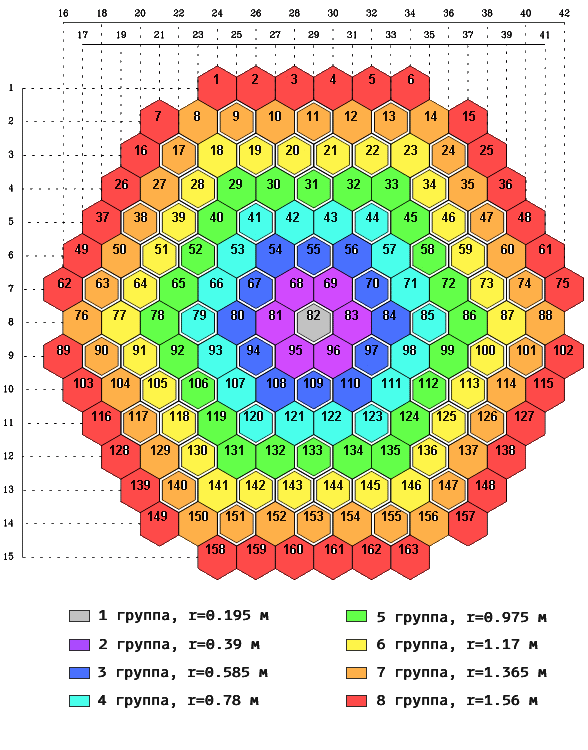
\includegraphics[scale=0.7]{treton_cells.png}
		\caption{Картограмма ячеек моделируемой АЗ для расчетного кода «ТРЕТОН» и их разбиение на группы по радиусу}
		\label{pic:treton-kartogramma}
	\end{center}
\end{figure}


Для каждой зоны были расчитаны тепловыделения, нормируя на соответствующие $K_r^i$, $K_z^j$, где $i = \overline{1, 8}$, $j = \overline {1, 30}$.

Распределение $K_r$ по группам было подобрано ориентируясь на следующие зависимости:
\begin{equation}
    K_r(r) \sim J_0(\frac{\xi_0 r}{R_{\text{эфф}}}) \approx - \alpha r^2 + \beta
\end{equation}, распределение коэффициента неравномерности по радиусу в приближении параболической функции
\begin{equation}
    \label{equation:KriNi}
    \sum_{i=1}^{8} K_r^i N_i = N_{\text{ТВС}} \pm 0.01
\end{equation}, где $N_i$ — количество ТВС в $i$-той группе по радиусу – условие нормировки распределения коэффициента неравномерности по радиусу.
Коэффициент $\beta$ параболической функции был подобран из условия, что в центре $K_r(r=0)$ должна быть равна табличному значению $K_r$ из \ref{tabular:data}, коэффициент $\alpha$ для удовлетворения соотношения \ref{equation:KriNi}. Полученные значения распределения коэффициента неравномерности по радиусу для каждой группы представлены в таблице \ref{tabular:Kri}.

\begin{figure}[H]
	\begin{center}
		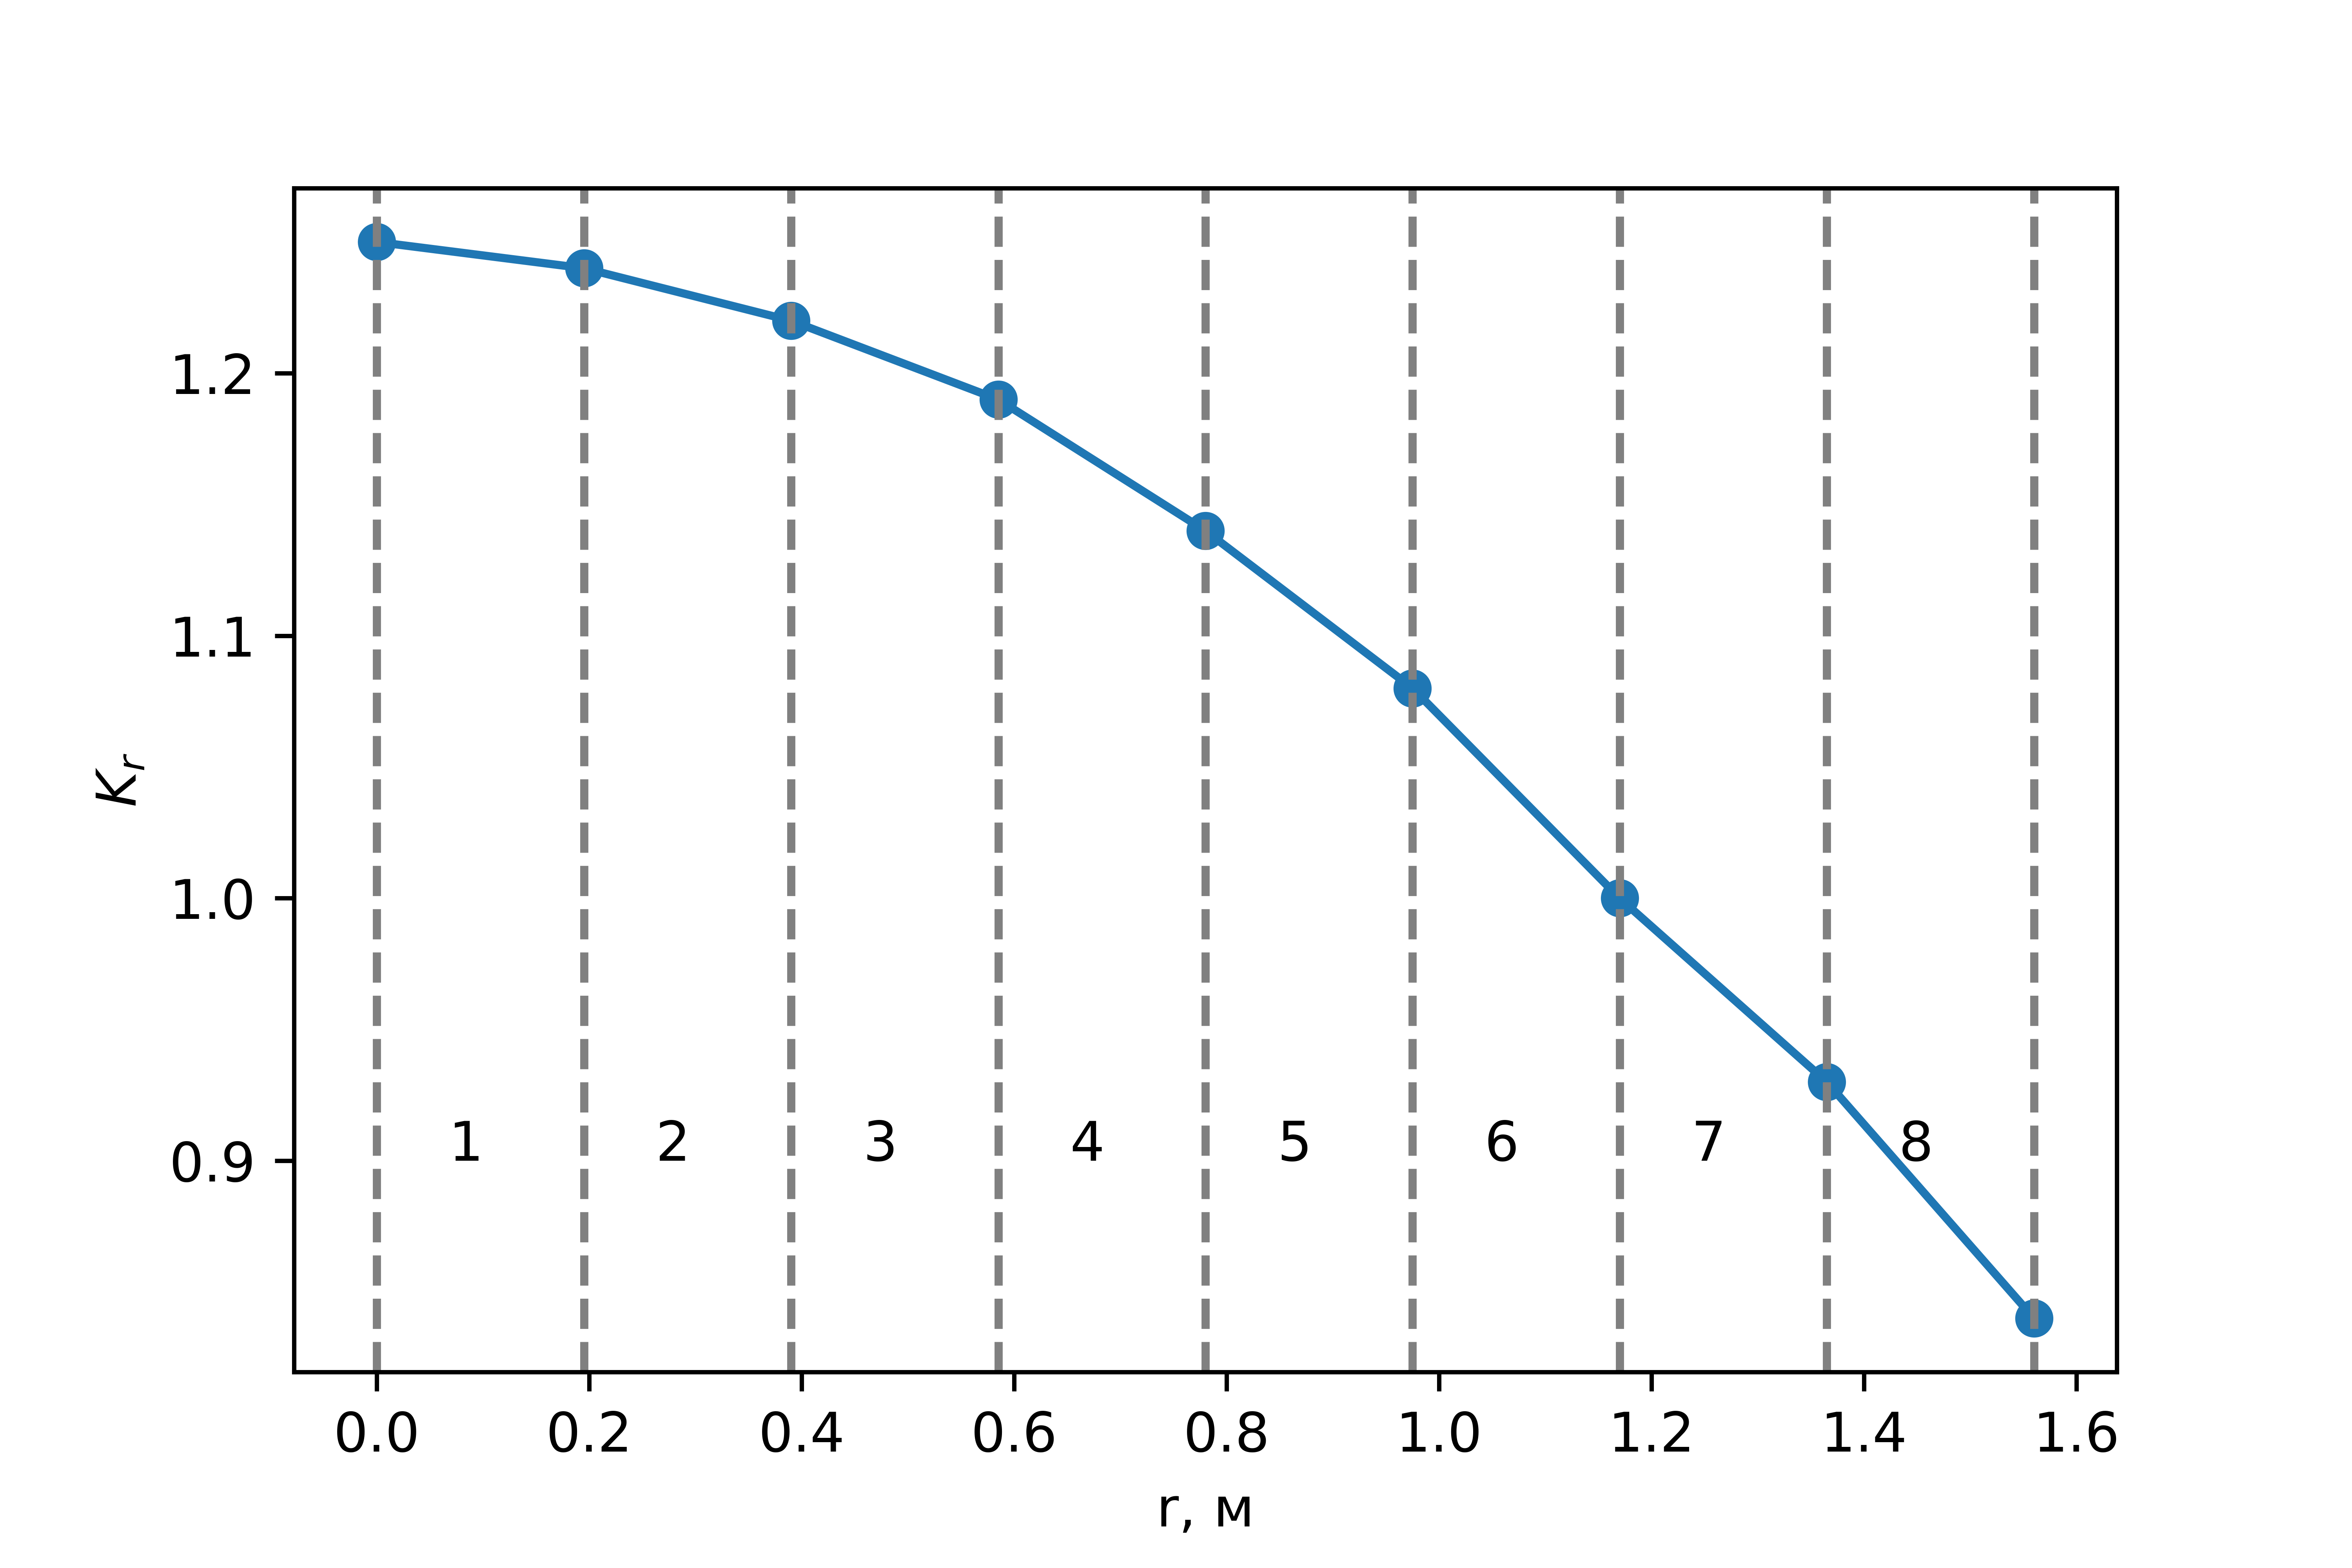
\includegraphics[scale=0.8]{Kr.png}
		\caption{Распределение коэффициента неравномерности по радиусу для восьми групп ТВС}
		\label{pic:Kr}
	\end{center}
\end{figure}

\begin{table}[H]
	\caption{Коэффициент неравномерности энерговыделения по радиусу для групп ТВС}
	\begin{center}
        \begin{tabular}{|l|c|}
        \toprule
         Номер группы & Значение $K_r^i$ \\
         \midrule
         \hline
         1 & 1.24 \\
         \hline
         2 & 1.22 \\
         \hline
         3 & 1.19 \\
         \hline
         4 & 1.14 \\
         \hline
         5 & 1.08 \\
         \hline
         6 & 1.00 \\
         \hline
         7 & 0.93 \\
         \hline
         8 & 0.84 \\
         \bottomrule
		\end{tabular}
		\label{tabular:Kri}
	\end{center}
\end{table}


\noindent Распределение коэффициента неравномерности по высоте $K_z$ определяется как:
\begin{equation}
    K_z(z) = K_z \cos \left( \frac {\pi z} {H_{\text{эфф}}} \right)
\end{equation}
где $z = \overline{-H_{\text{АЗ}} / 2,\  H_{\text{АЗ}} / 2}$ м.


\noindent Распределение $K_z$ по высоте представлено на рис \ref{pic:Kz}


\begin{figure}[H]
	\begin{center}
		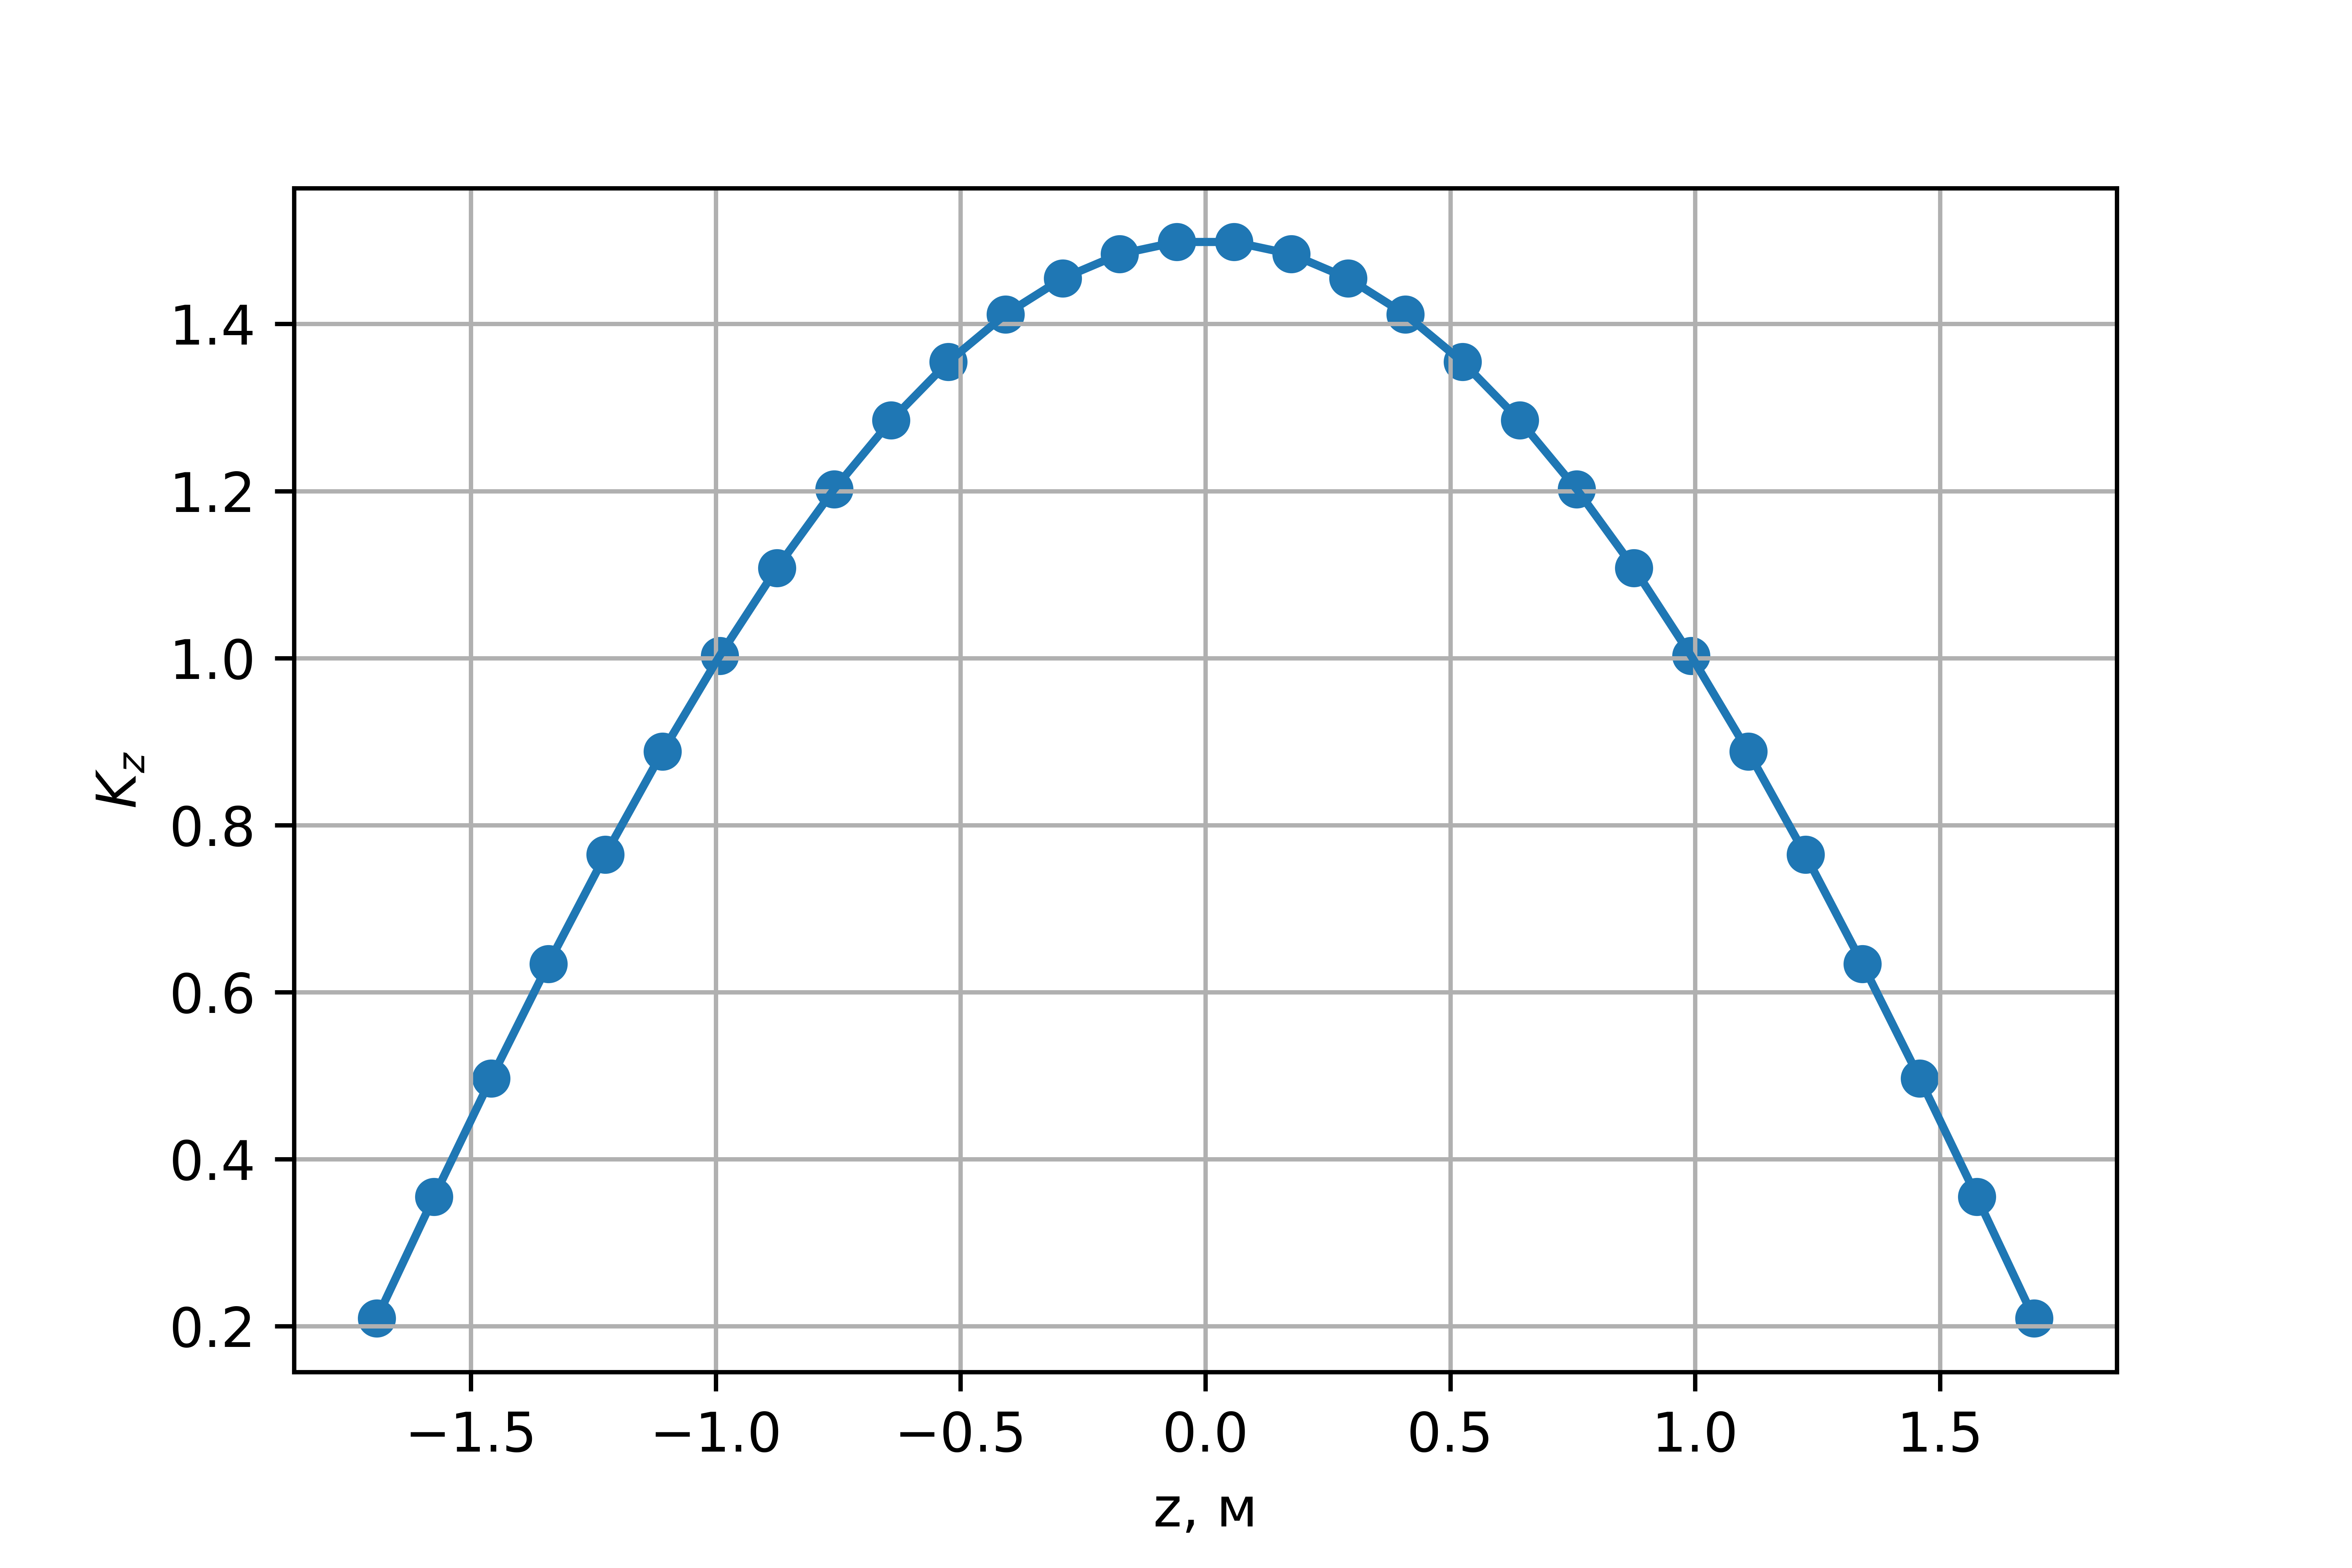
\includegraphics[scale=0.8]{Kz.png}
		\caption{Распределение коэффициента неравномерности по высоте активной зоны}
		\label{pic:Kz}
	\end{center}
\end{figure}


Из полученных распределений $K_r$, $K_z$ было определено распределение тепловыделения для всех групп расчетных элементов
\begin{align}
    \label{equation:Qzr}
    Q(z, r) &= K_z(z)K_r(r)\frac{Q_{\text{теп}}}{N_{\text{ТВС}} \cdot 30} \\
            &= K_r(r) K_z \cos \left( \frac{\pi z}{H_{\text{эфф}}} \right) \frac{Q_{\text{теп}}}{N_{\text{ТВС}} 30}
\end{align}

На основе соотношения \ref{equation:Qzr} был сформирован входной файл \texttt{Q6.txt} с тепловыделением для всех расчетных элементов в соответствии с картограммой \ref{pic:treton-kartogramma}

Далее были проведены калибровочные расчеты для определения входных параметров файла \texttt{THEHYCO.INI}, соответствующих проектируемой РУ. Основным критерием выбора параметров было соответсвие вычисленному программой «ТРЕТОН» расходу полученному ранее в рамках теплофизического расчета.

Таким образом расчетным кодом было получено значение расхода $G_{\text{расч}} = (1.570 \pm 0.016) \cdot 10^4\  \frac{\text{кг}}{\text{с}}$, что соответствует полученному ранее значению $G_{\text{реак}} = 1.579 \cdot 10^4\ \frac{\text{кг}}{\text{с}}$ в пределах погрешности. 
Значения входных параметров файла \texttt{THETHYCO.INI}, при которых достигнут такой расход приведены в таблице \ref{tabular:thethyco_nominal}

\begin{table}[H]
    \caption{Входные параметры расчета при номинальном режиме работы}
    \begin{center}
        \begin{tabular}{|l|c|}
        \toprule
        Параметр & Значение \\
        \midrule
        \hline
        Шаг твэлов, мм & 12.75 \\ 
        \hline
        Поперечный размер расчетной области, м & 0.241 \\
        \hline
        Продольный размер расчетной области, м & 0.118 \\
        \hline
        Кол-во твэлов в ТВС, шт & 317 \\
        \hline
        Расчетный дисбаланс & 0.005 \\
        \hline
        Входное давление, Па & 15800000 \\
        \hline
        Выходное давление, Па & 15686938 \\
        \bottomrule
        \end{tabular}
		\label{tabular:thehyco_nominal}
    \end{center}
\end{table}

% TODO: табличка с параметрами THEHYCO.INI по разделам с именами

% \begin{table}[H]
% 	\caption{wow}
% 	\begin{center}
%         \begin{tabular}{|l|c|}
%         \toprule
%          Раздел RodList & \\
%          \midrule
%          \hline
%          tmp=0.75 3.86 4.25 4.55 & разбиение твэлов на контрольные объемы, указаны радиусы центрального отверстия твэла, границы топливного столба, центра оболочки, внешней границы оболочки. мм\\
%          \hline
%          $\texttt{s_mesh}$=12.75 & шаг твэлов, мм \\
%          \hline
%          d\_mesh=9.1 & диаметр твэла, мм \\
%          \hline
%         %  $\texttt{R_contact}$=0.00024 & контактное сопротивление толиво-оболочка, $\text{м}^2 \cdot \text{К} / \text{Вт}$ \\
%         %  \hline
%          Раздел HEATandHYDROlist & \\
%          \midrule
%          \texttt{dr}=0.241 & поперечный размер расчетной области, м\\
%          \hline
%          \texttt{dz}=0.118 & продольный размер расчетной области, м\\
%          \hline
%          $\texttt{n_RodsInTVS}$ =317 & количество твэлов в ТВС \\
%          \hline
%          \texttt{Disbalance}=0.001 & расчетный дисбаланс \\
%          \hline
%          $\texttt{p_input}$=15800000 & входное давление, Па \\
%          \hline
%          $\texttt{p_output}$=15691054 & выходное давление,  Па \\
%          \bottomrule
% 		\end{tabular}
% 		\label{tabular:thehyco_nominal}
% 	\end{center}
% \end{table}

На основе описанных входных параметров был произведен расчет с шагом по времени $dt=0.0005$ для 100 итераций. По результату расчета были построены зависимости основных теплогидравлических параметров и сопоставлены со значениями, полученными в теплофизческом расчете.

По итогам расчета на основе результатов файла \texttt{t\_tepl.dat} была построено распределение температуры теплоносителя по высоте активной зоны, усредненное по всем расчетным элементам. График распределения вместе с распределением теплоносителя по высоте, рассчитанном в рамках теплофизического расчета \ref{pic:Tz} представлен на рисунке \ref{pic:treton-t-tepl-compare-teplofiz}.

\begin{figure}[H]
	\begin{center}
		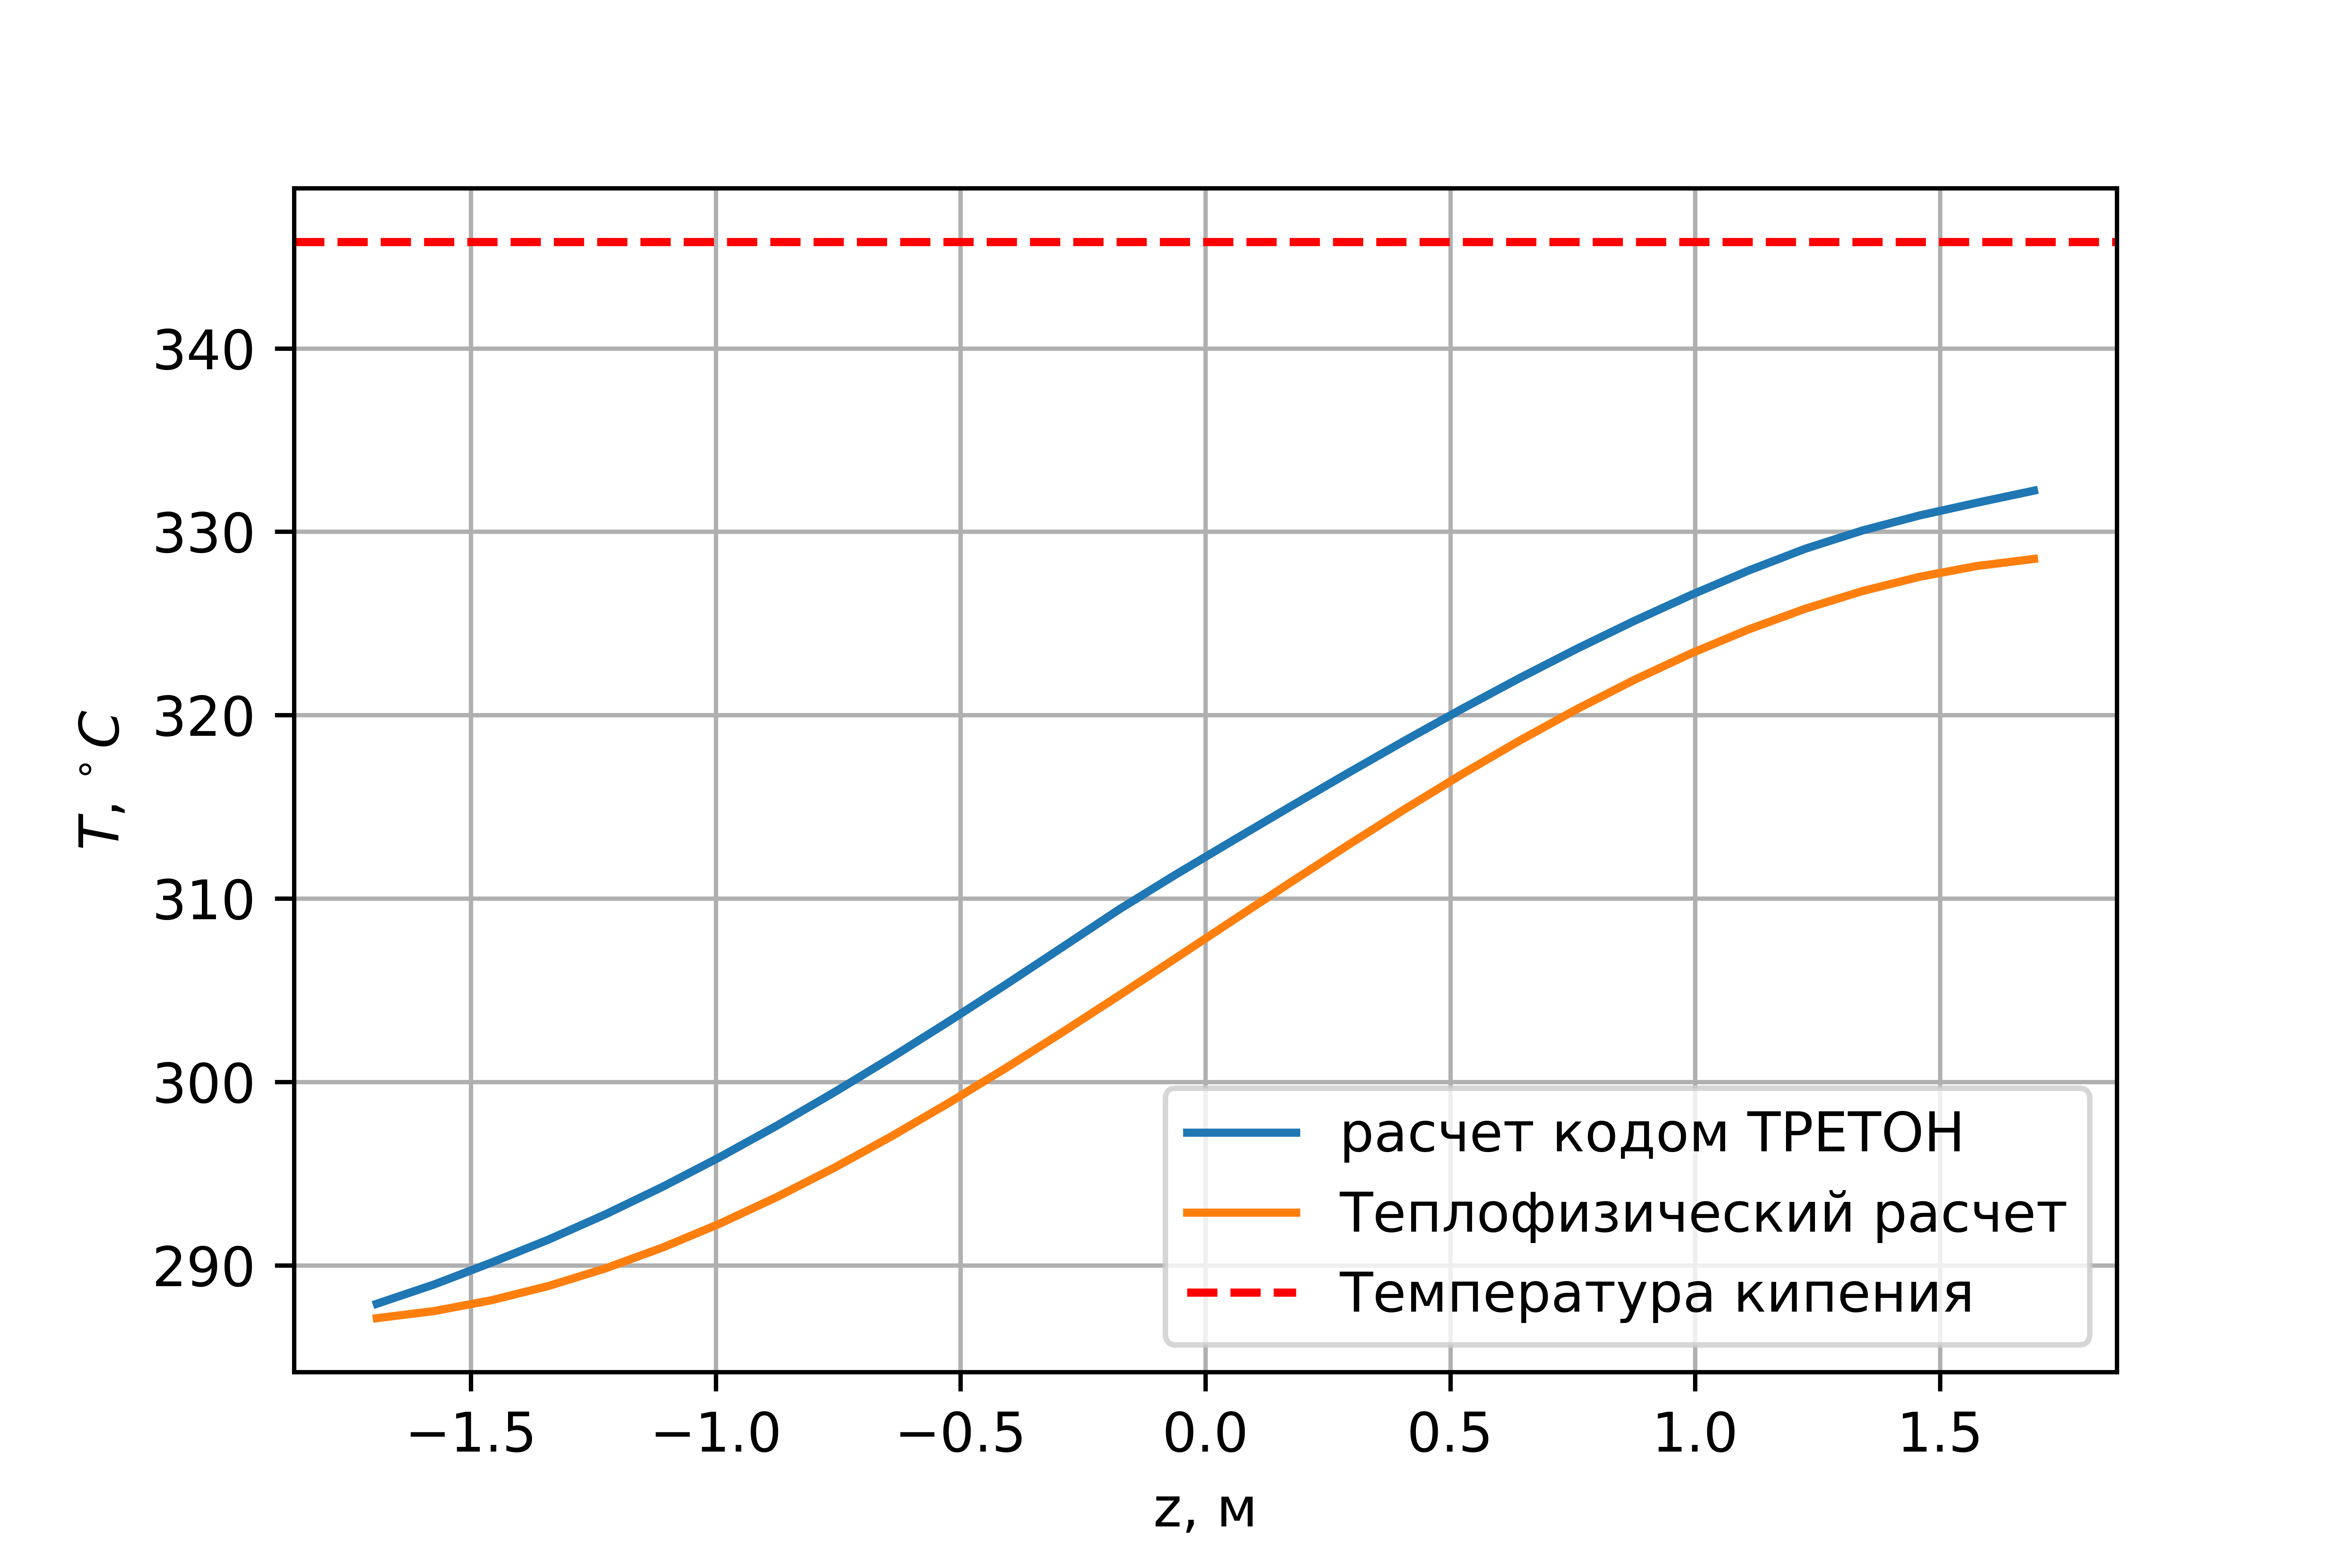
\includegraphics{treton_nominal_t_z.png}
		\caption{Распределение температуры теплоносителя по высоте}
		\label{pic:treton-t-tepl-compare-teplofiz} % название для ссылок внутри кода
	\end{center}
\end{figure}

Из рис \ref{pic:treton-t-tepl-compare-teplofiz} видно, что отклонение максимального значения температуры на выходе из активной зоны полученного в рамках расчета программой ТРЕТОН от значения полученного теплофизическим расчетом составляет -0.08\%. Среднеквадратичная ошибка составляет $\Delta {T_{\text{теп}}} = 1.8 ^\circ C$. Отсюда мы можем сделать вывод о соответствии полученных результатов ранее рассчитанным в рамках приемлемой погрешности.

Для номинального режима работы реактора были построены распределения температуры теплоносителя по высоте для каждой рассматриваемой групп и для кассеты, с максимальной температурой на выходе из активной зоны. Распределения представлены на рисунках \ref{pic:treton-t-tepl-nominal-by-r}, \ref{pic:treton-t-tepl-nominal-max}

\begin{figure}[H]
	\begin{center}
		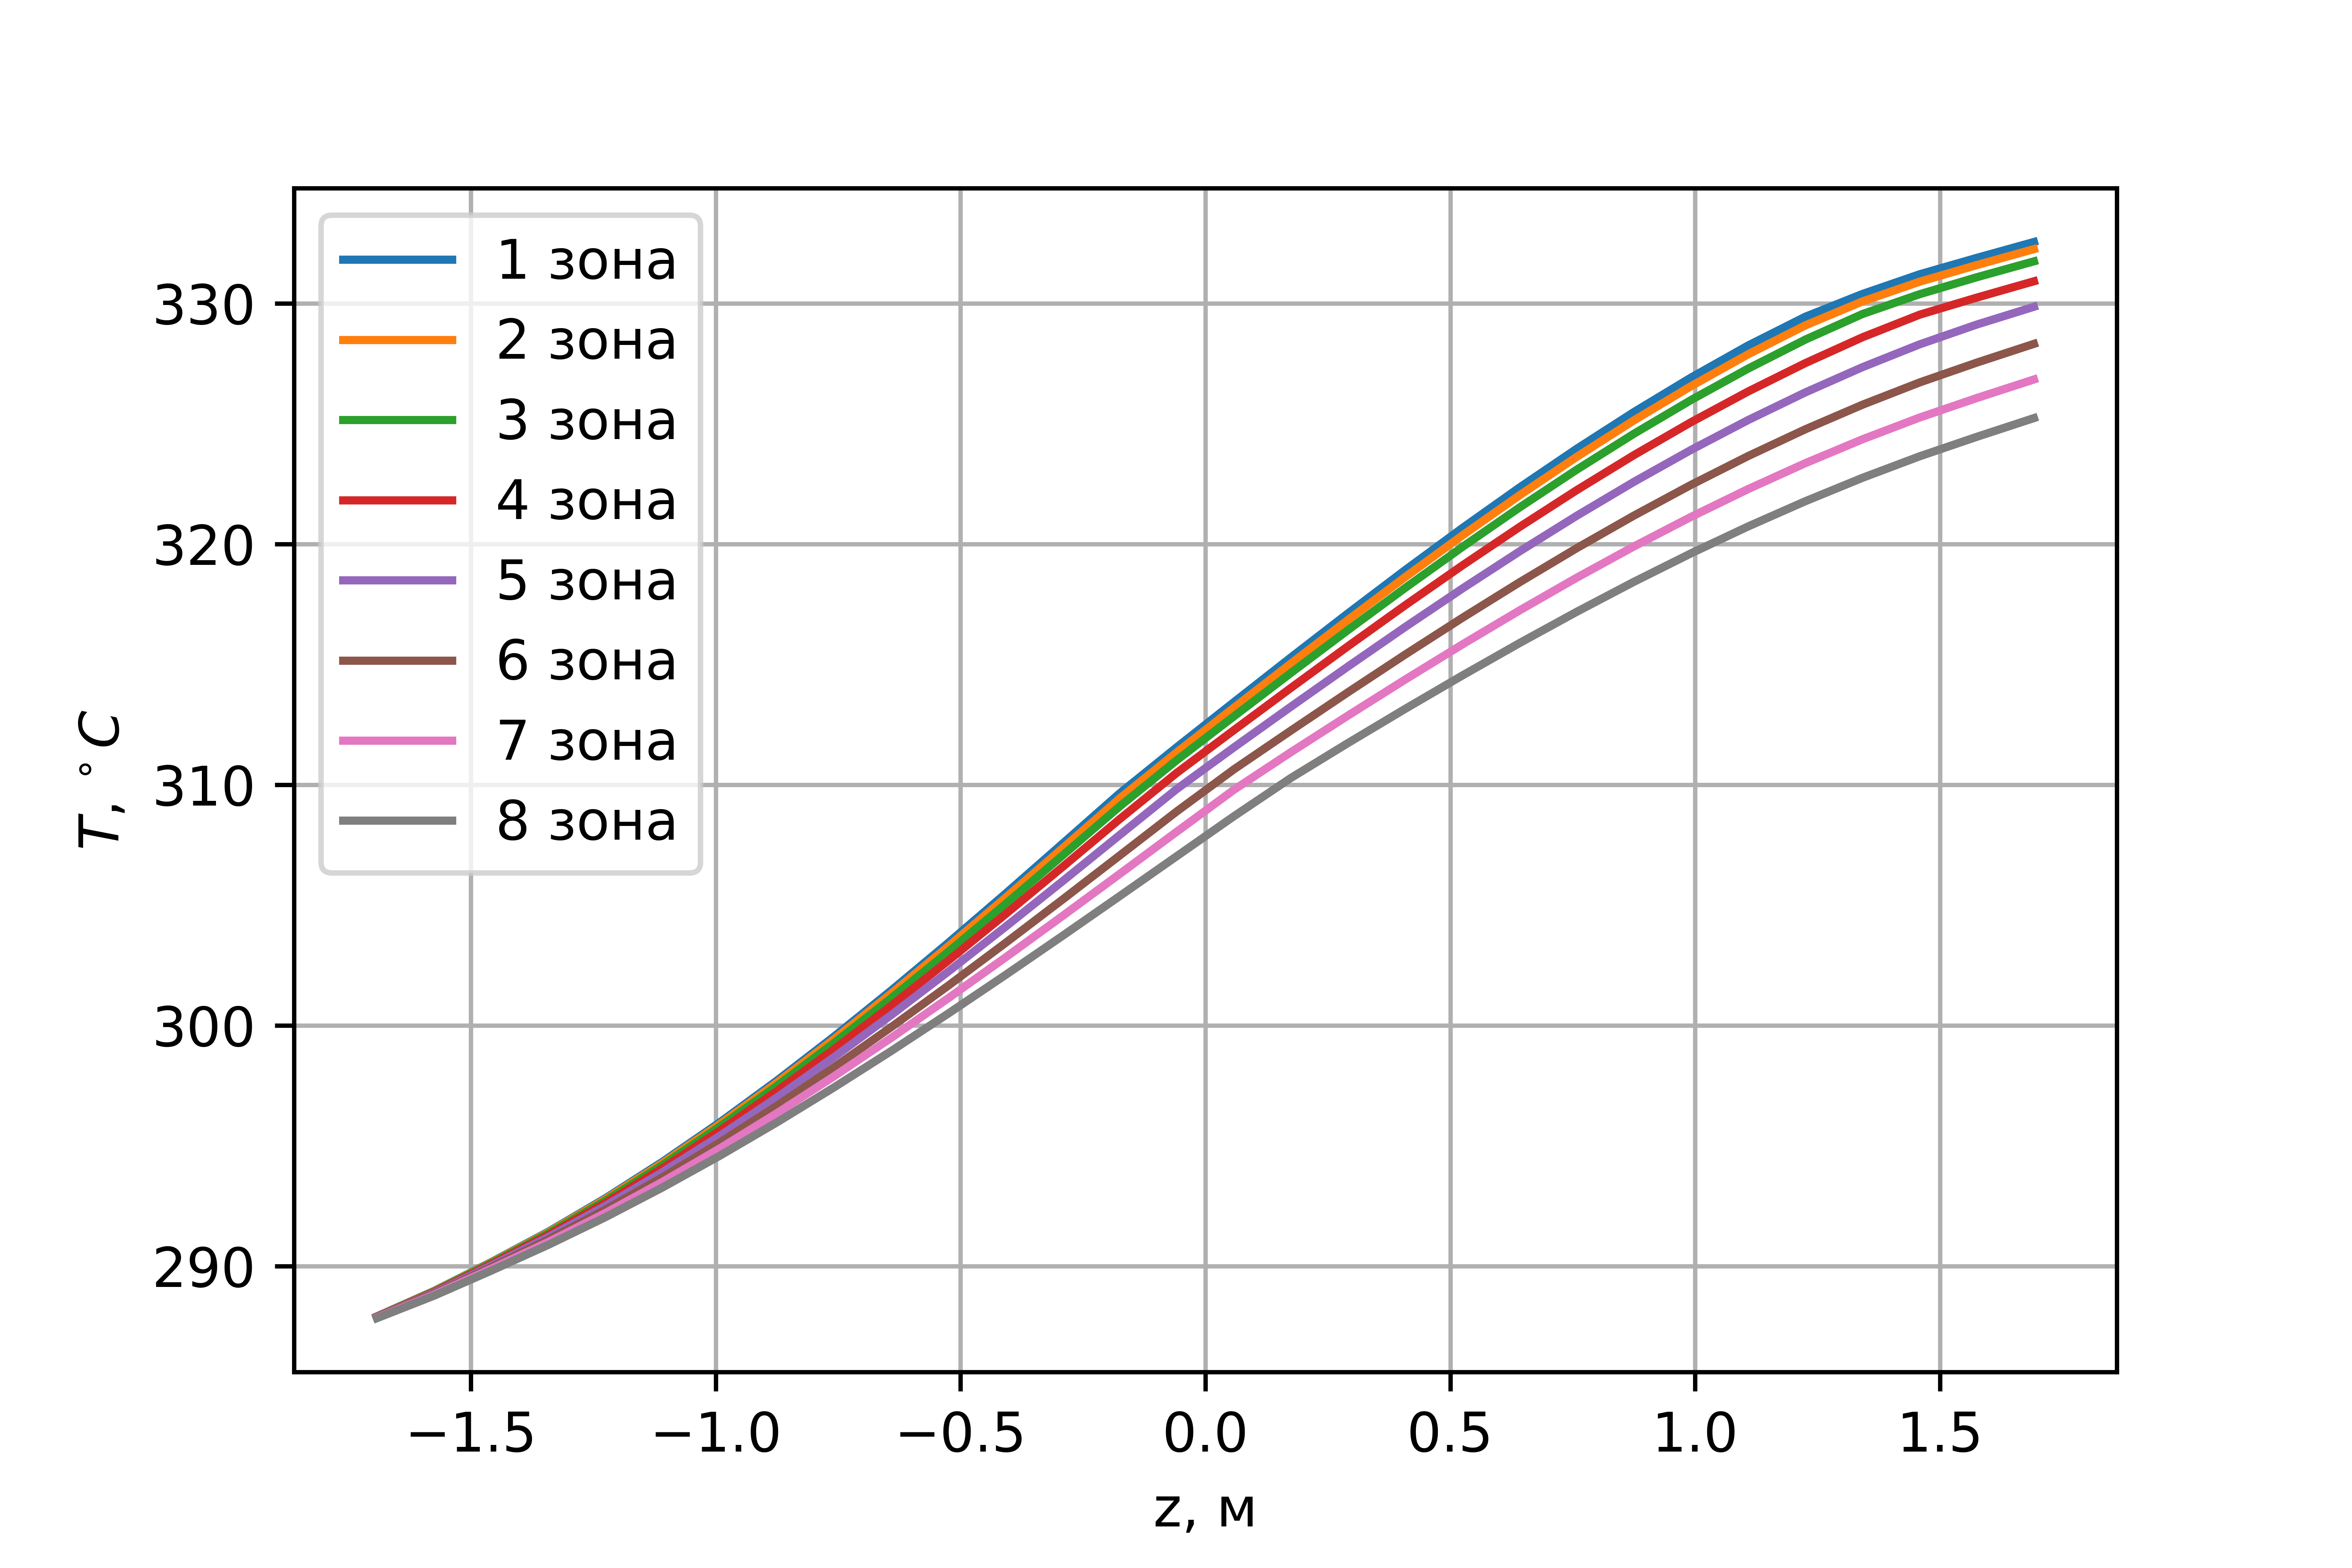
\includegraphics{treton_nominal_t_z_by_r.png}
		\caption{Распределение температуры теплоносителя по высоте для каждой зоны по радиусу}
		\label{pic:treton-t-tepl-nominal-by-r} % название для ссылок внутри кода
	\end{center}
\end{figure}

\begin{figure}[H]
	\begin{center}
		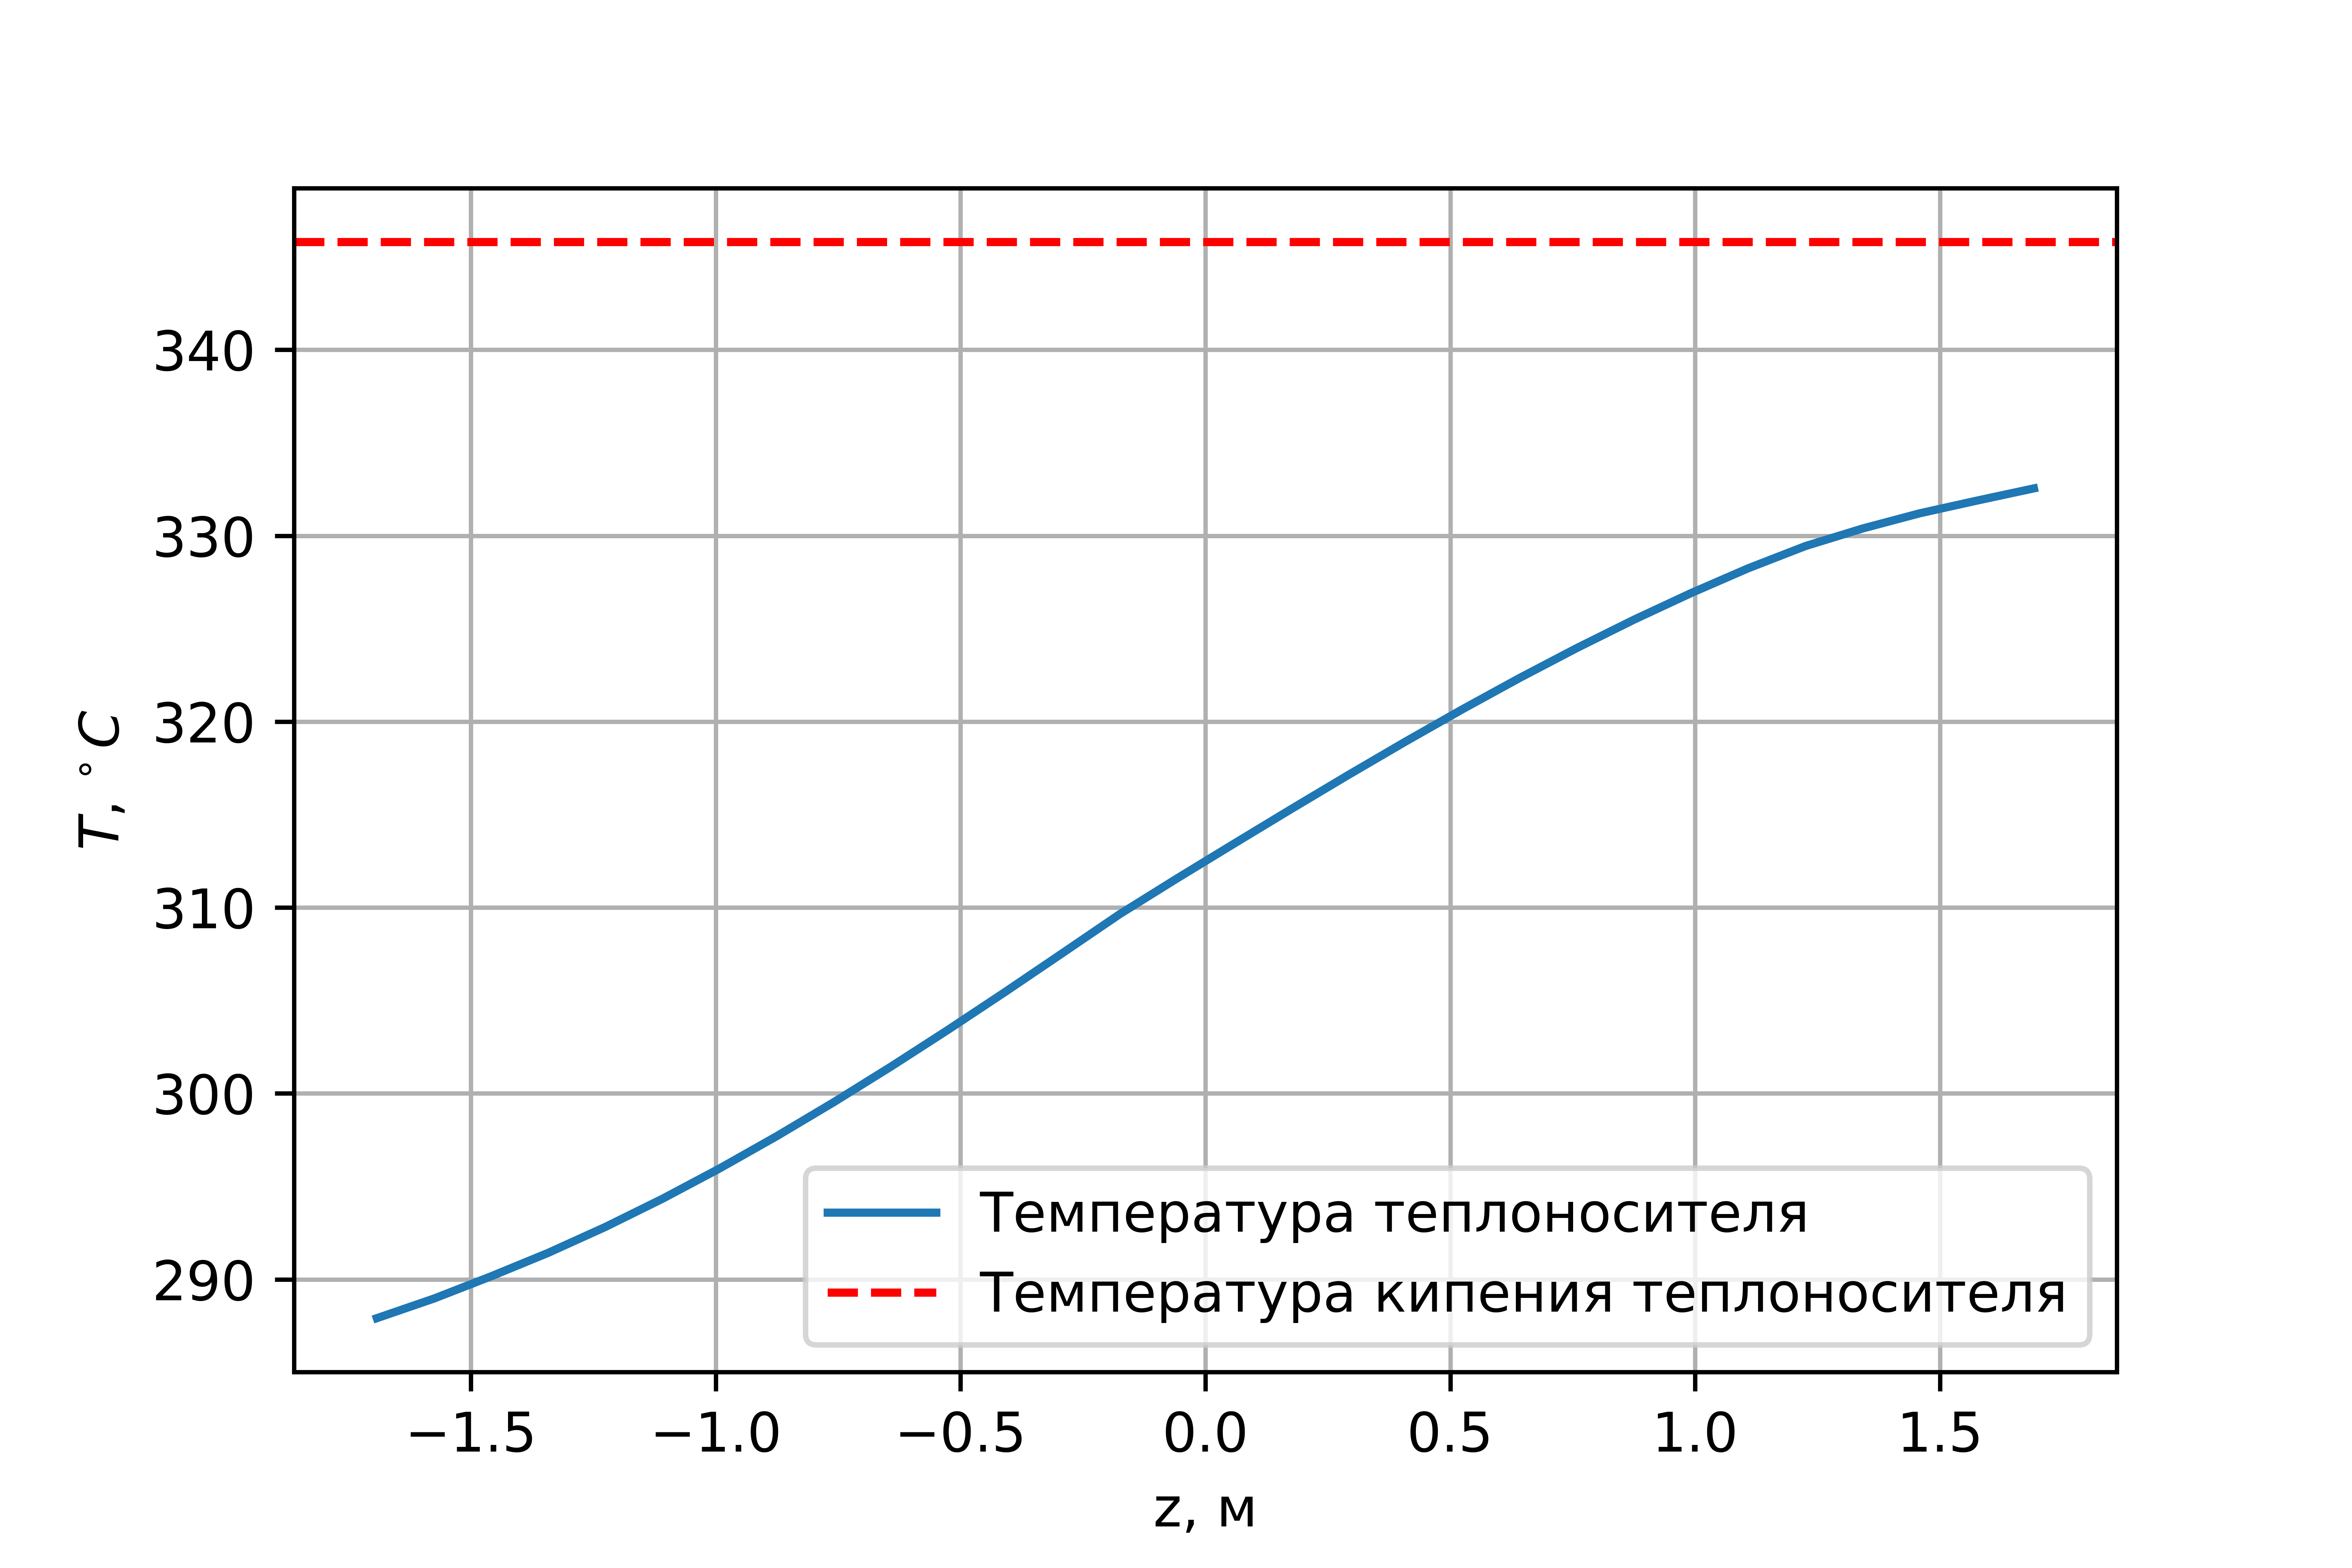
\includegraphics{treton_nominal_t_z_max.png}
		\caption{Распределение температуры теплоносителя по высоте для кассеты с максимальной температурой на вызоде из АЗ}
		\label{pic:treton-t-tepl-nominal-max} % название для ссылок внутри кода
	\end{center}
\end{figure}

 Из \ref{pic:treton-t-tepl-nominal-max} видно, что максимальная температура теплоносителя $T_{\text{тепл} \text{Ном}}^{\max} = 332.5 ^\circ C$.
 При рассматриваемом давлении в активной зоне 15.8 МПа температура кипения теплоносителя составляет $346.5\ ^\circ C$, отсюда следует что запас до кипения составляет $13.65 ^\circ C$

 Для топлива были получены распределения температуры топлива по высоте активной зоны для ячейки с максимальной температурой топлива в центре АЗ и распределение температуры топлива по высоте АЗ для всех групп по радиусу. Зависимости представлены на рисунках \ref{pic:treton-t-fuel-nominal-max}, \ref{pic:treton-t-fuel-nominal-by-r}

\begin{figure}[H]
	\begin{center}
		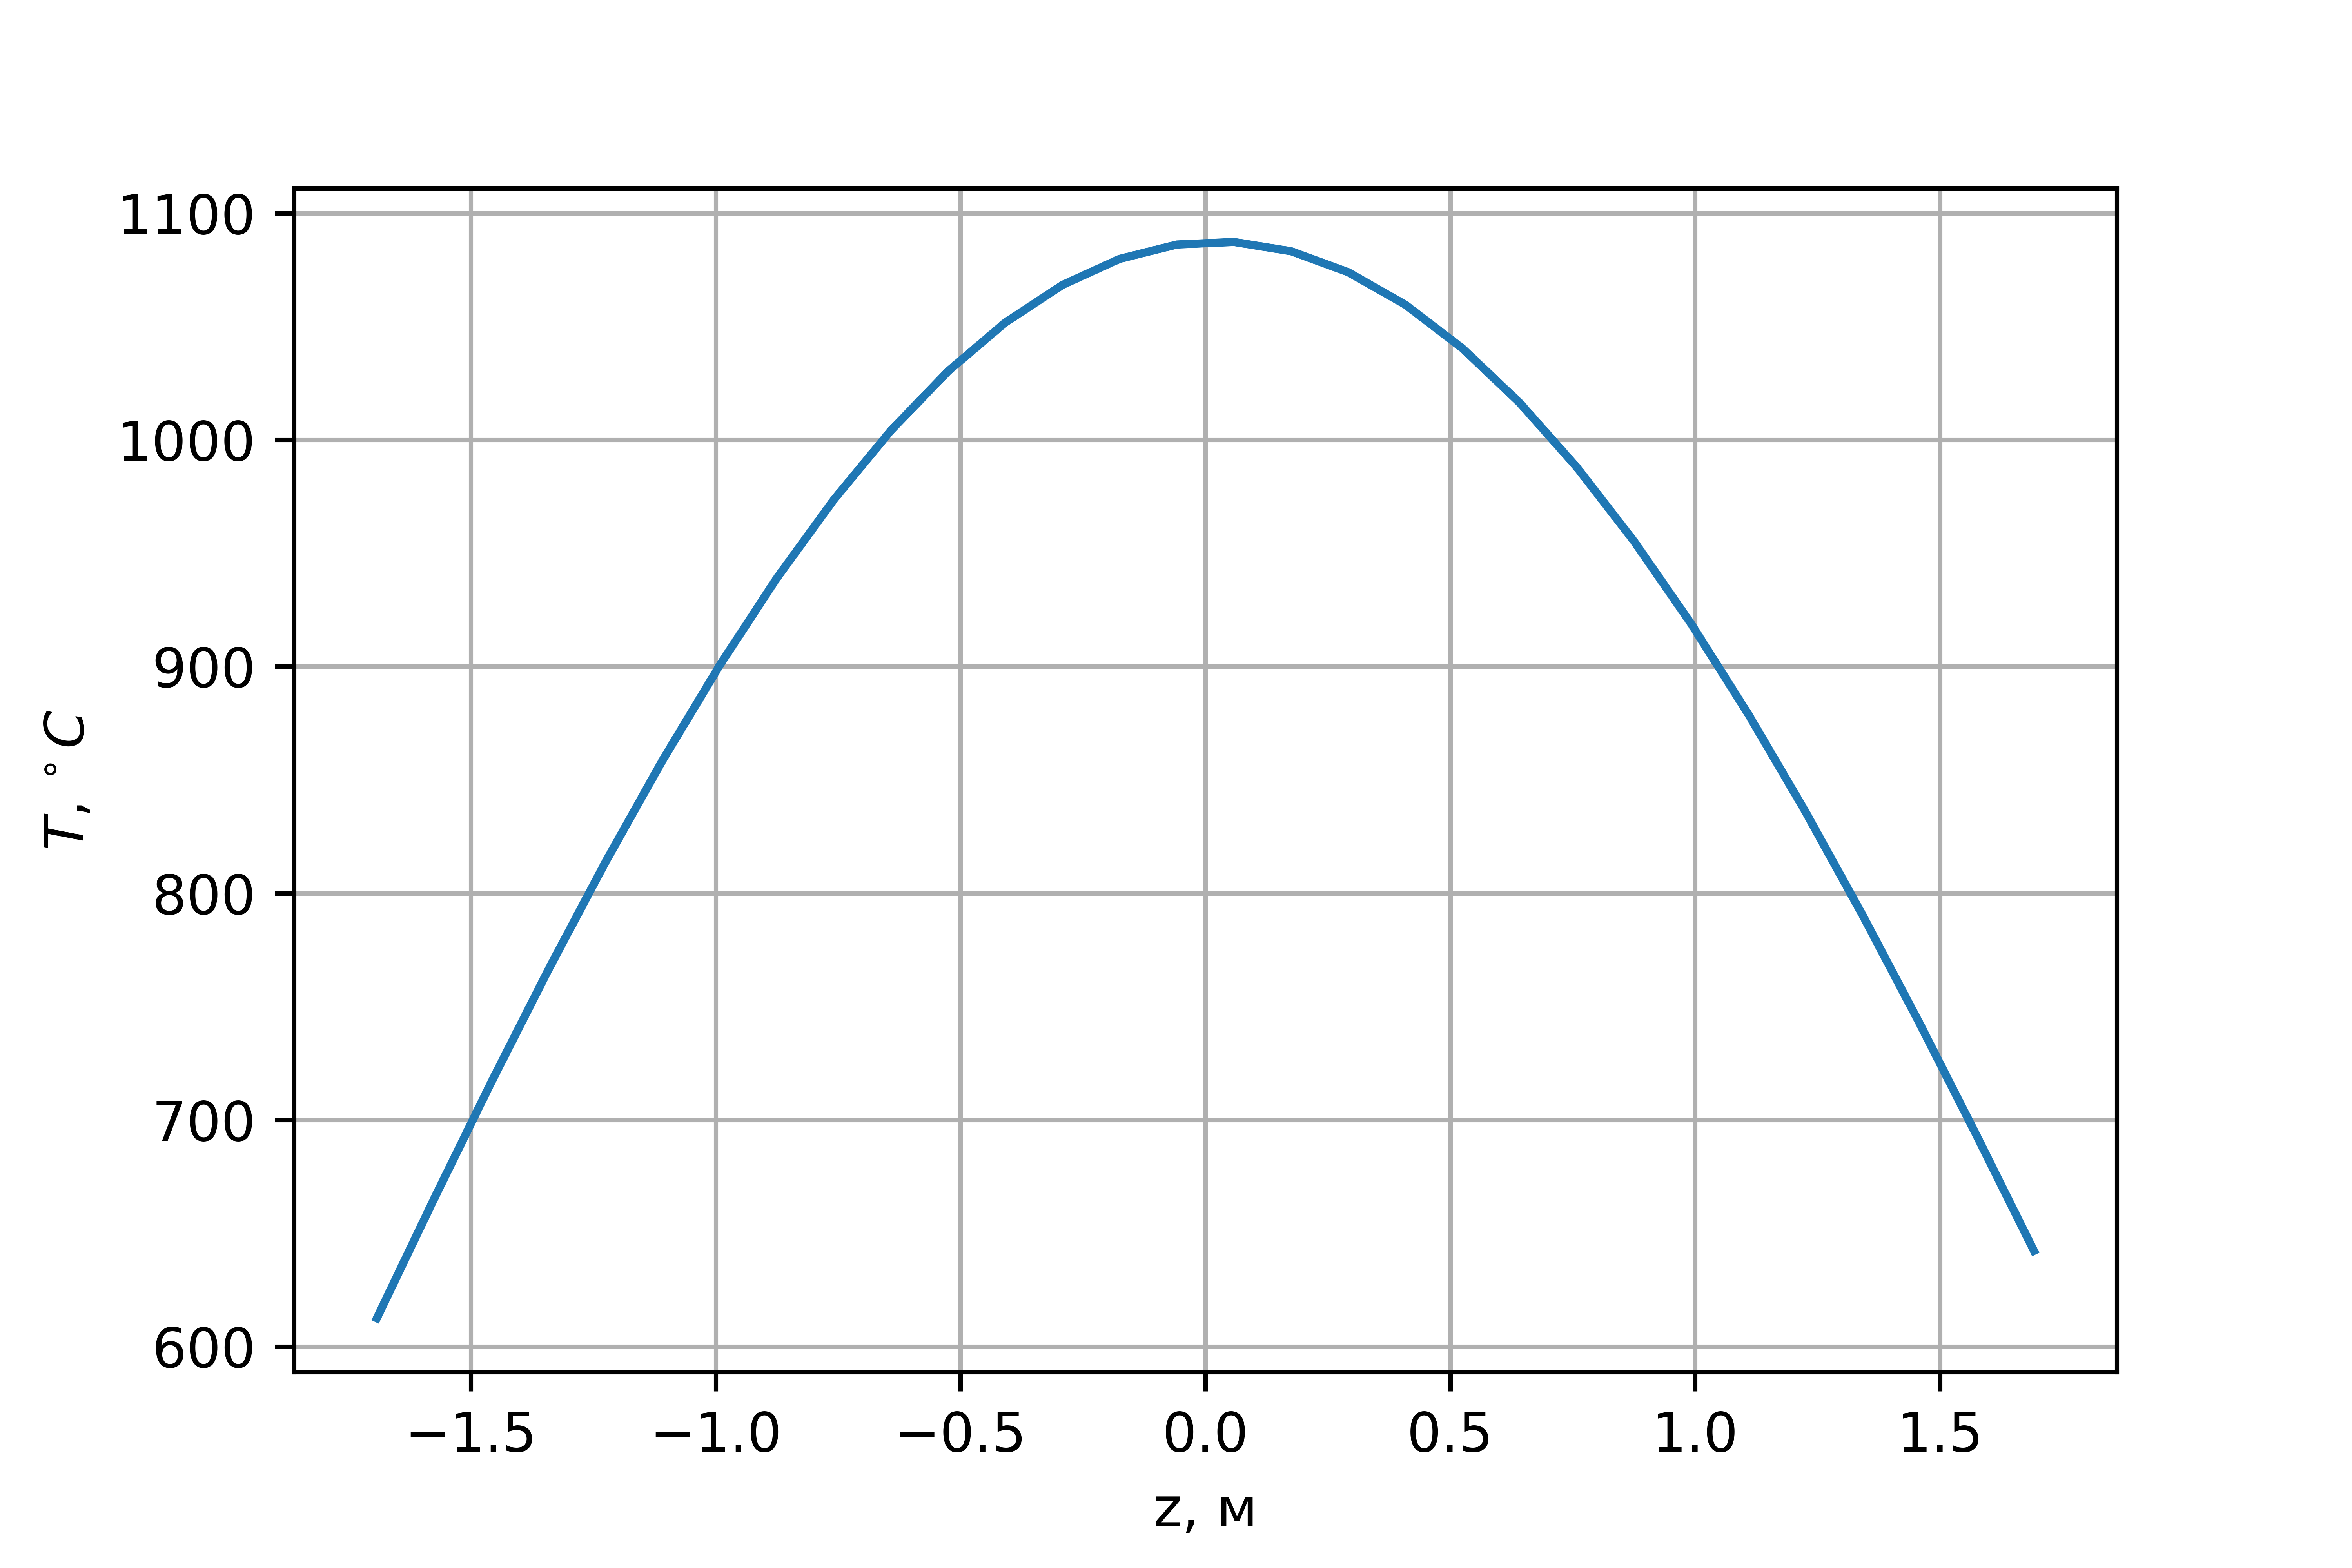
\includegraphics{treton_nominal_t_fuel_max.png}
		\caption{Распределение температуры топлива по высоте АЗ для кассеты с максимальной температурой топлива в центре АЗ}
		\label{pic:treton-t-fuel-nominal-max} % название для ссылок внутри кода
	\end{center}
\end{figure}

\begin{figure}[H]
	\begin{center}
		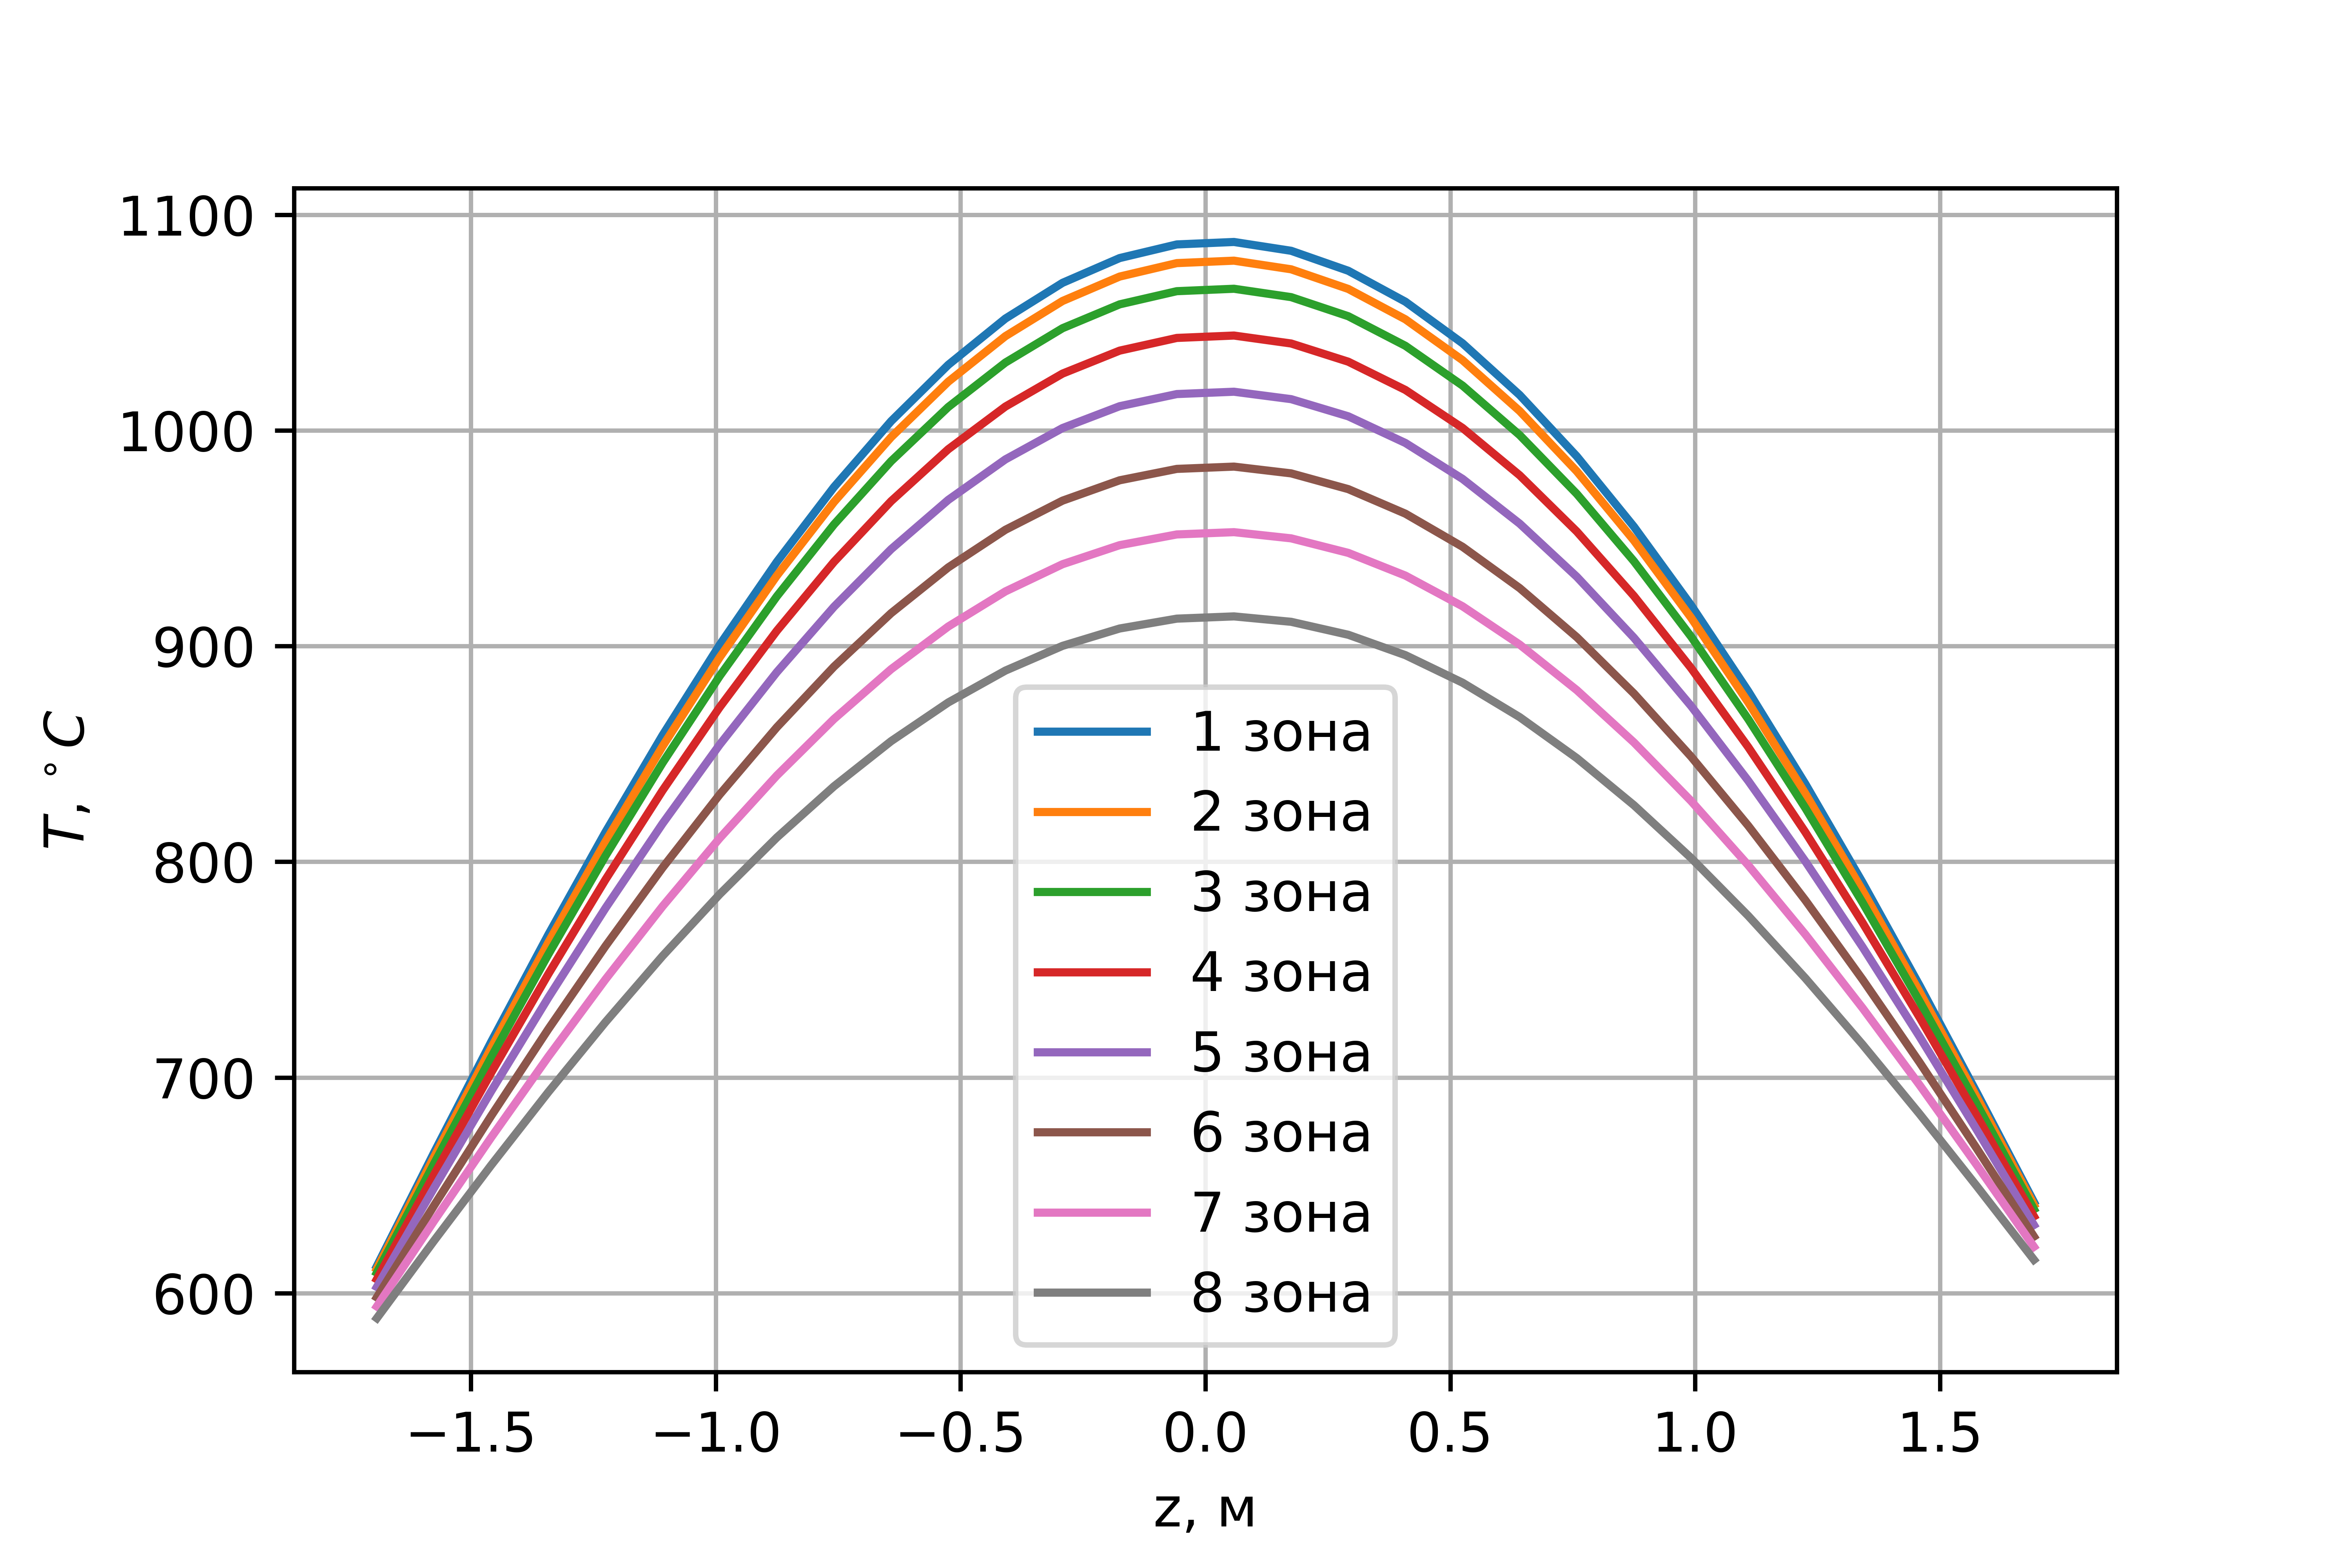
\includegraphics{treton_nominal_t_fuel_by_r.png}
		\caption{Распределение температуры топлива по высоте для всех групп по радиусу АЗ}
		\label{pic:treton-t-fuel-nominal-by-r} % название для ссылок внутри кода
	\end{center}
\end{figure}

Из графиков видно, что максимальная температура топлива
$T_{\text{топ} \text{Ном}}^{\max} = 1087.4 ^\circ C$, что не превышает максимально допустимую при авариях температуру плавления оксида урана $2600 ^\circ C$

Для ячейки с максимальной температурой также были построены зависимости температуры оболочек от высоты активной зоны. Из рис \ref{pic:treton-t-obl-naruj-nominal-max} максимальная температура оболочки составляет $346.46 ^\circ C$, запас до кипеня теплоносителя около стенки составляет $0.04, ^\circ C$, из чего можно сделать вывод что пристеночное кипения не наблюдается

\begin{figure}[H]
	\begin{center}
		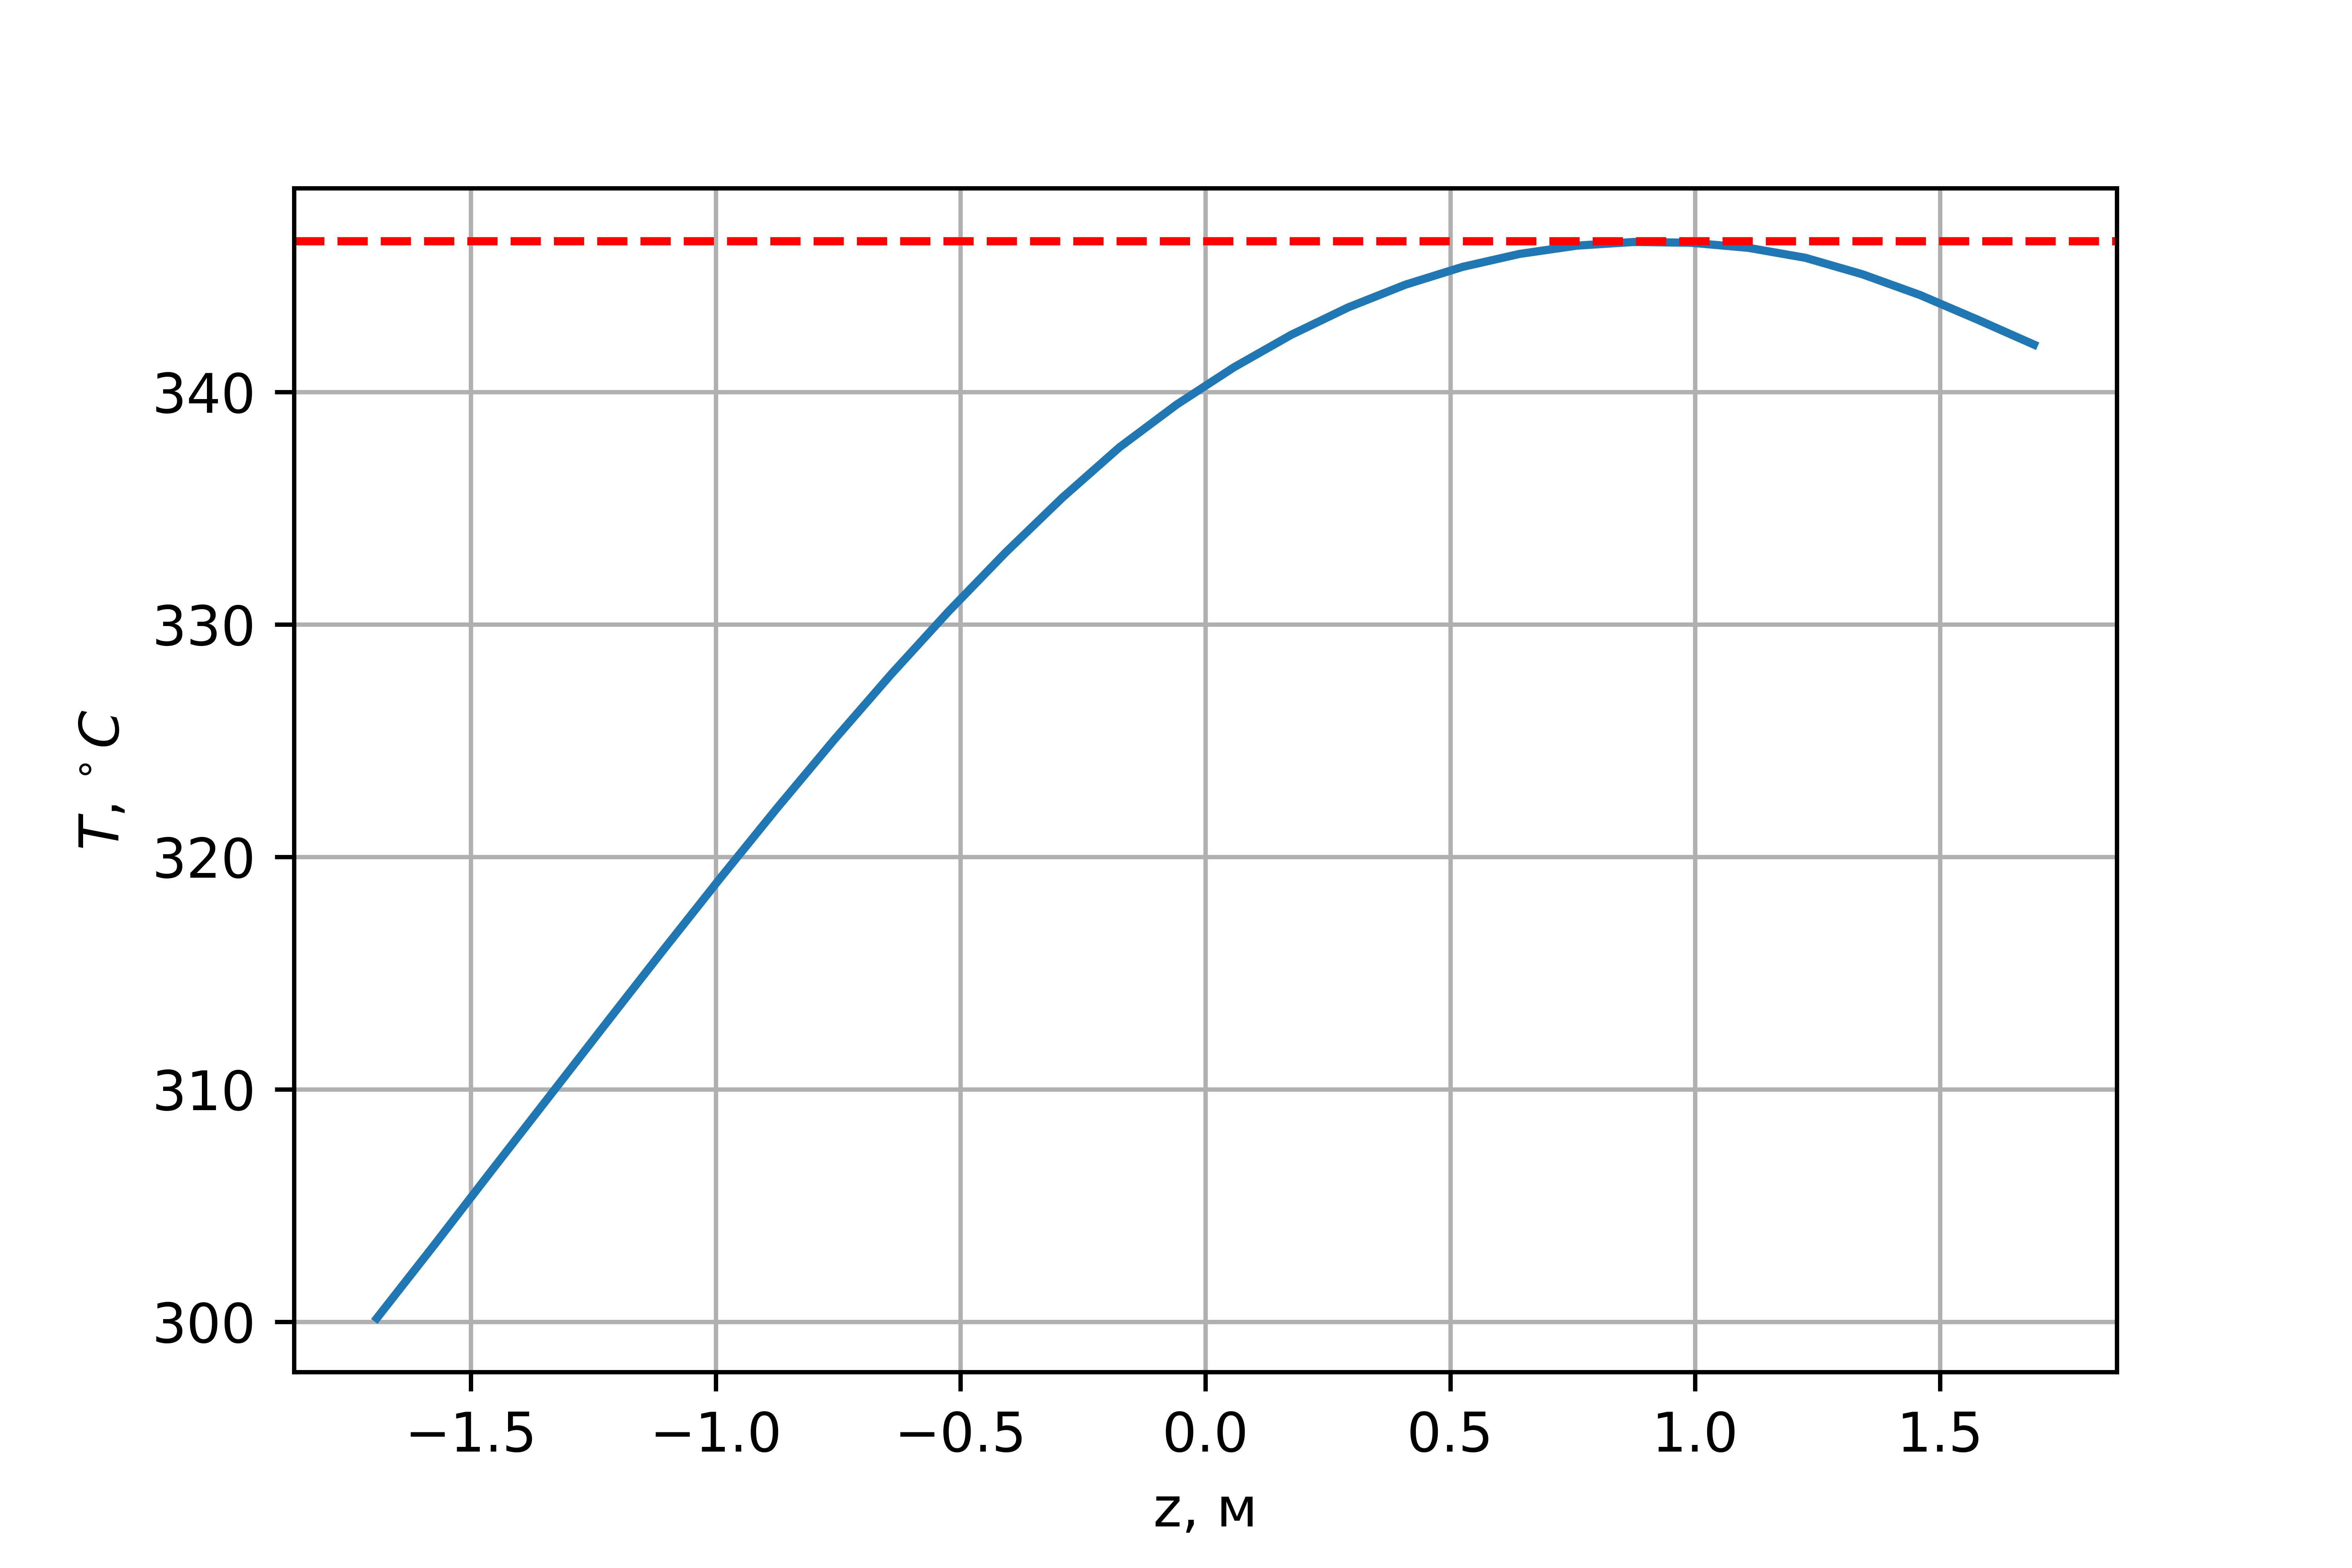
\includegraphics{treton_nominal_obl_naruj_max.png}
		\caption{Распределение температуры внешней оболочки по высоте для кассеты с максимальной температурой на выходе из АЗ}
		\label{pic:treton-t-obl-naruj-nominal-max} % название для ссылок внутри кода
	\end{center}
\end{figure}

На рис \ref{pic:treton-obl-tepl-obsh-nominal} представлен  общий график для распределения температур наружней, внутренней оболочки и теплоносителя

\begin{figure}[H]
	\begin{center}
		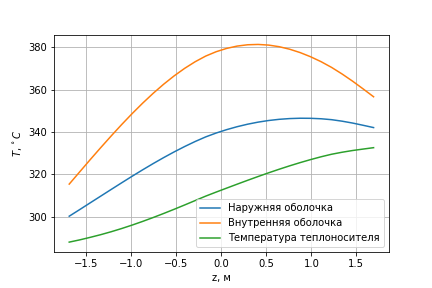
\includegraphics{treton_nominal_obl_tepl_obsh.png}
		\caption{Распределение температур оболочек и теплоносителя по высоте АЗ}
		\label{pic:treton-obl-tepl-obsh-nominal} % название для ссылок внутри кода
	\end{center}
\end{figure}

Для ячейки с максимальной температурой топлива на выходе также было построено распределение давления теплоносителя по высоте активной зоны, которое представлено на рисунке \ref{pic:treton-p-nominal-max}. Перепад давлений в кассете составляет 96.1 Па

\begin{figure}[H]
	\begin{center}
		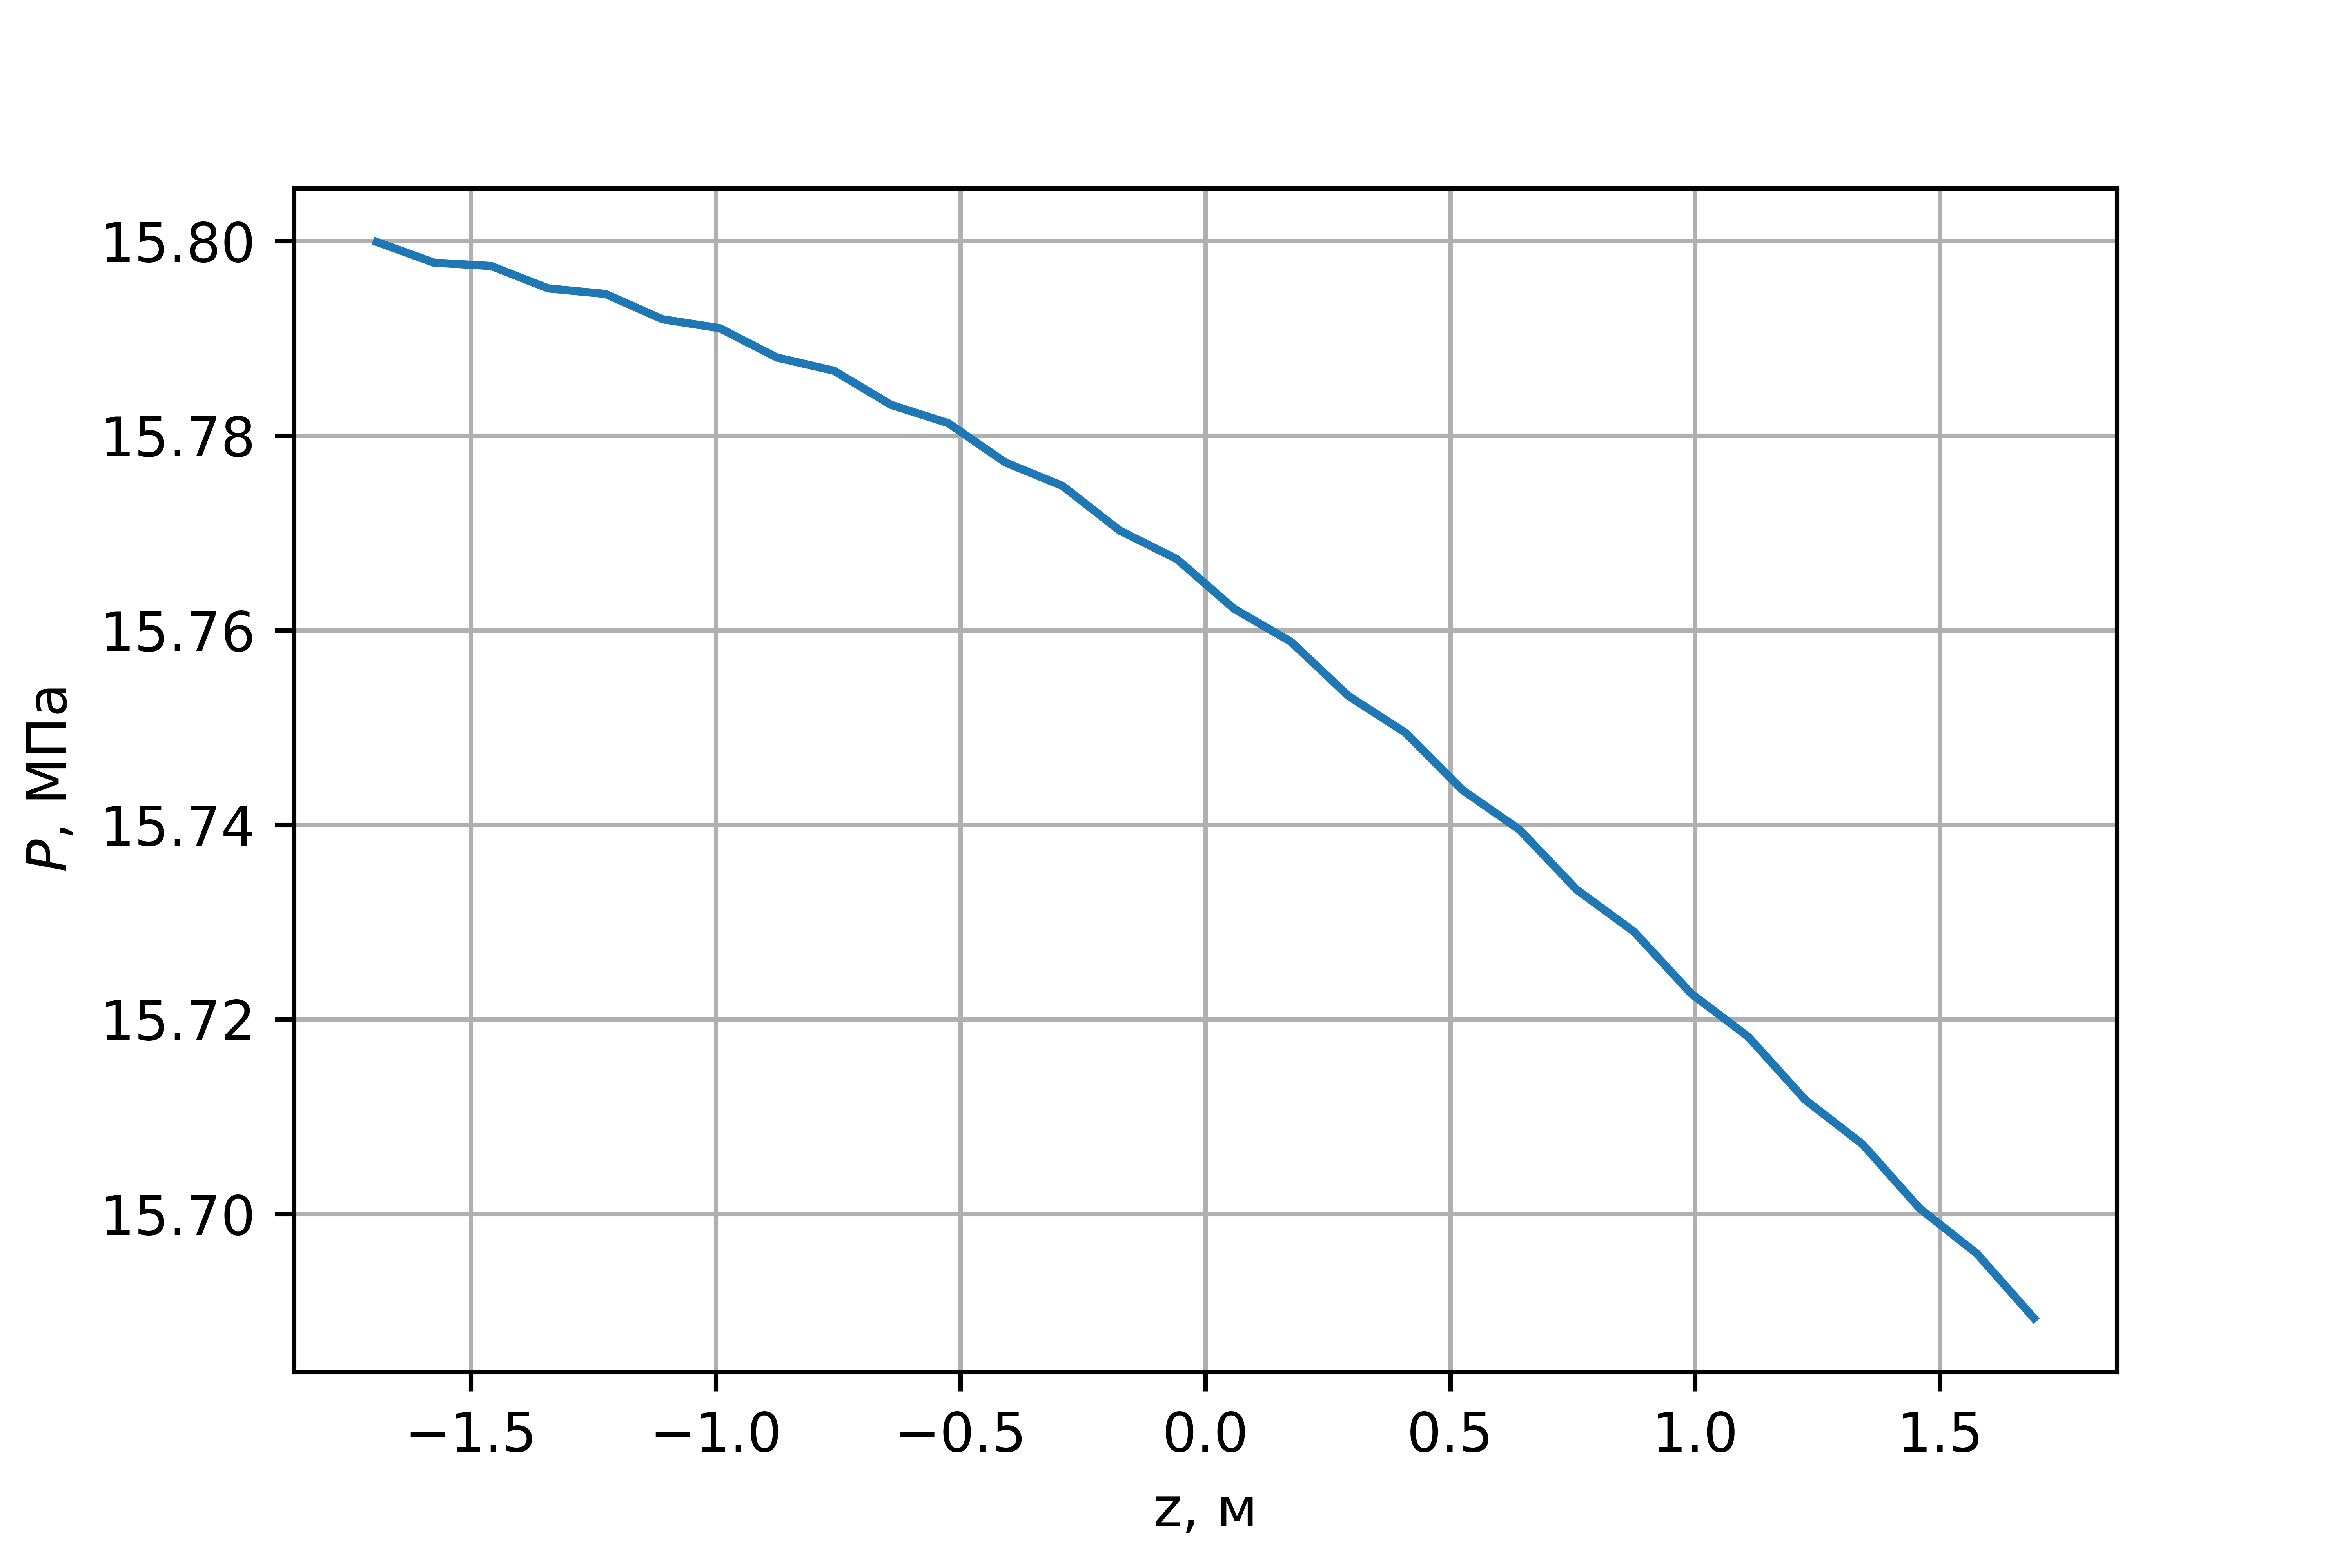
\includegraphics{p_nominal_max.png}
		\caption{Распределение давления в кассете с максимальной температурой на выходе по высоте активной зоны}
		\label{pic:treton-p-nominal-max} % название для ссылок внутри кода
	\end{center}
\end{figure}

Для каждой ТВС были расчитаны подогревы теплоносителя. На \ref{pic:treton-podogrev-nominal} представлено распределение подогрева по каждой кассете ТВС, на \ref{pic:treton-podogrev-nominal-by-r} усредненное распределение по радиальным группам ТВС в соответствии с разбиением представленным на картограмме \ref{pic:treton-kartogramma}.


\begin{figure}[H]
	\begin{center}
		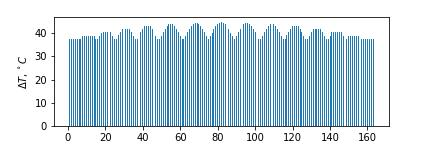
\includegraphics[scale=0.5]{podogrev_nominal.jpg}
		\caption{Распределение подогревов ТВС}
		\label{pic:treton-podogrev-nominal} % название для ссылок внутри кода
	\end{center}
\end{figure}

\begin{figure}[H]
	\begin{center}
		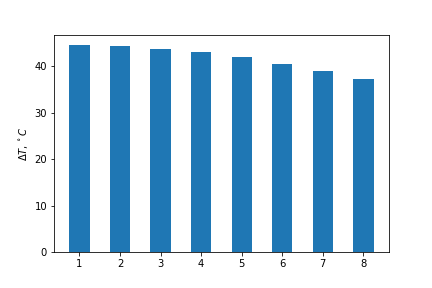
\includegraphics{podogrev_nominal_by_r.png}
		\caption{Распределение подогревов ТВС усредненное по группам}
		\label{pic:treton-podogrev-nominal-by-r} % название для ссылок внутри кода
	\end{center}
\end{figure}

% TODO: график расхода

\subsection{Расчет теплогидравлических характеристик при работе на повышенной мощности}
Ввиду наличия успешных практик перевода работы реакторов ВВЭР-1000 на повышенную мощность для расматриваемой реакторной установки были выполнены теплогидравлические расчеты програмным комплексом «ТРЕТОН»
при работе реактора на мощности $115\% N_{\text{ном}}$ и номинальном значении температуры на входе активную зону. Для моделирования такого режима работы полученная зависимость тепловыделения от радиуса и высоты для номинального режима \ref{equation:Qzr} была промасштабирована коэфициентом 1.15:


\begin{equation}
	Q_{115 \% N_{\text{ном}}}(z,r) 
	= 1.15 \cdot Q(z,r) 
	= K_r(r) K_z \cos \left( 
		\frac{\pi z}{H_{\text{эфф}}} 
	  \right) 
	  \frac{1.15 \cdot Q_{\text{теп}}}{N_{\text{ТВС}} 30}
\end{equation}


Полученные максимальные значения температур теплоносителя, оболочек и топлива в сравнении с номинальным режимом работы представлены в таблице \ref{tabular:t_max_nominal_compare}. Распределения соответствующих температур по высоте представлены на рисунках \ref{pic:treton-t-fuel-povish-compare}, \ref{pic:treton-t-tepl-povish-compare}, \ref{pic:treton-povish-obl-naruj-max}. 

% TODO: таблица
% сразу графички в сравнении с температурами кипения

\begin{table}[H]
    \caption{Максимальные температуры теплоносителя, топлива и оболочки твэлов при работе РУ на номинальной и повышенной мощности}
    \begin{center}
        \begin{tabular}{|l|c|c|}
        \toprule
        Тепловая мощность, МВт & 2903 & 3339.2 \\
        \midrule
        \hline
        Максимальная температура теплоносителя, $\circ C$ & 332.5 & 336.3  \\ 
        \hline
        Запас до кипения теплоносителя, $\circ C$ & 13.9 &  10.17 \\
        \hline
        Максимальная температура топлива, $\circ C$ & 1087.4 & 1158.7  \\
        \hline
        Максимальная температура внешней оболочки & 346.46 & 349.4 \\
        \hline
        Максимальная температура внутренней оболочки & 381.3 & 389.7 \\
        \hline
        Запас до кипения теплоносителя вблизи оболоки & 0.04 & -2.9 \\
        \bottomrule
        \end{tabular}
		\label{tabular:t_max_nominal_compare}
    \end{center}
\end{table}

\begin{figure}[H]
	\begin{center}
		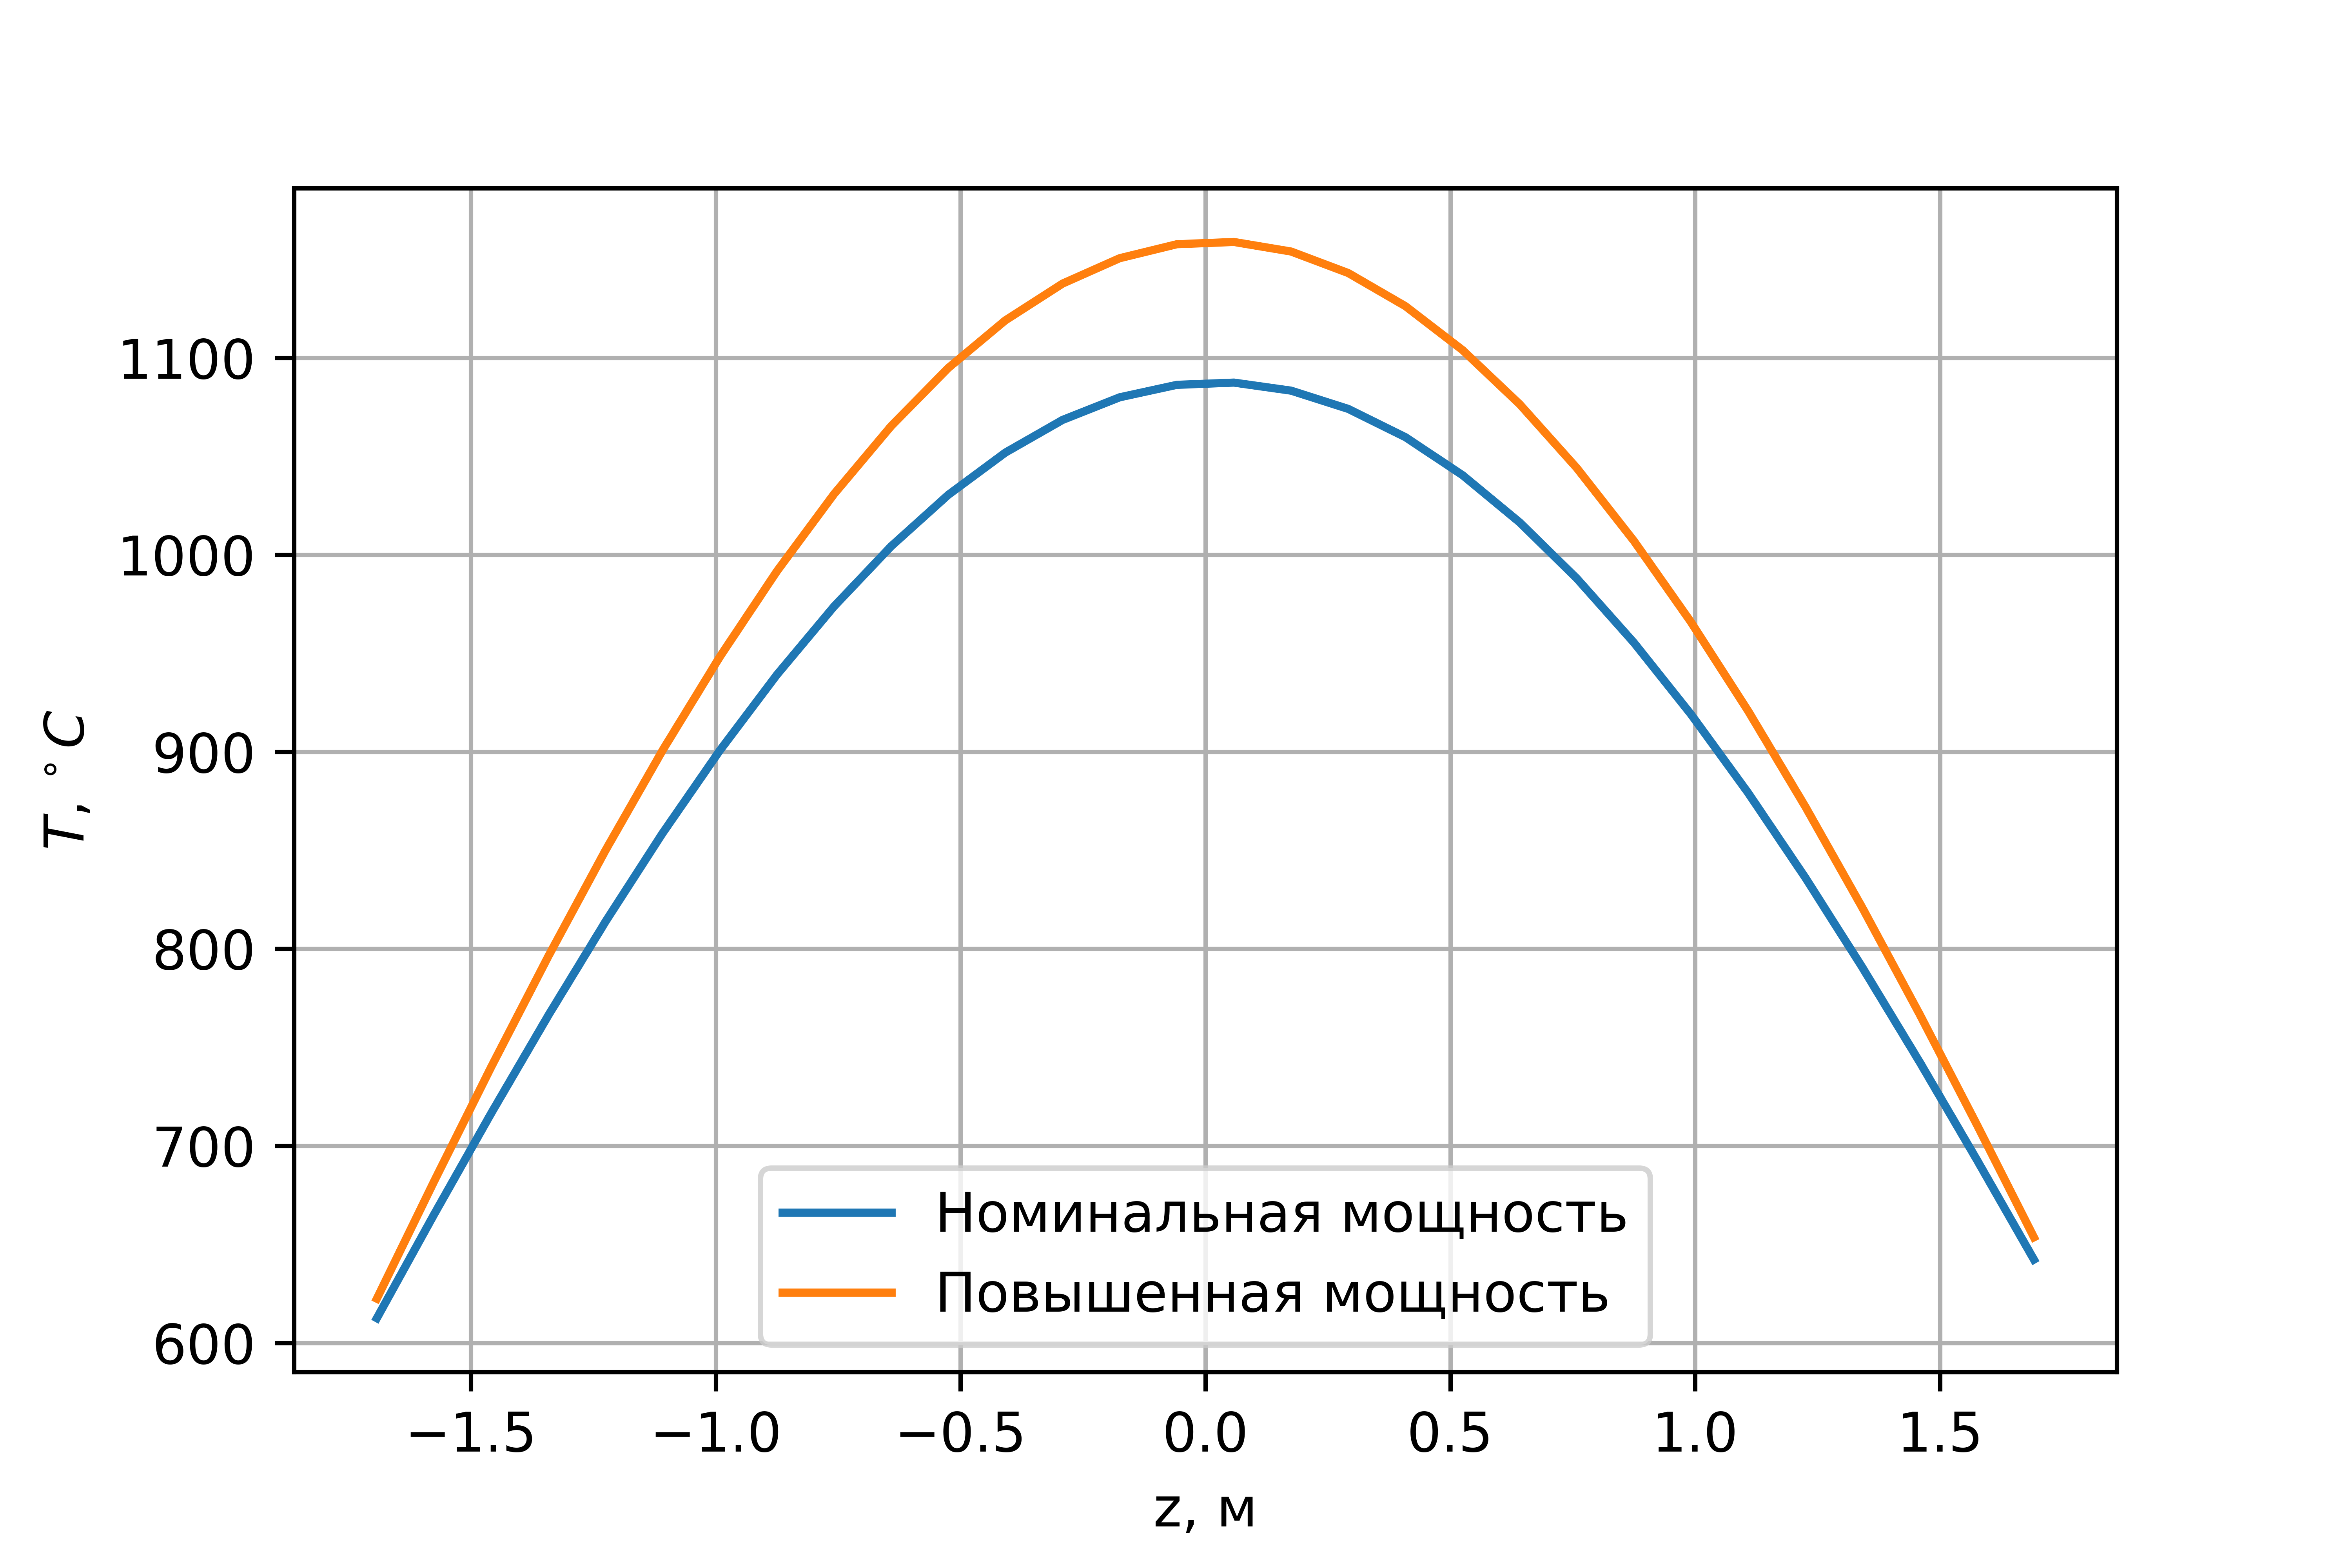
\includegraphics{treton_t_fuel_povish_compare.png}
		\caption{Распределение температуры топлива по высоте АЗ}
		\label{pic:treton-t-fuel-povish-compare} % название для ссылок внутри кода
	\end{center}
\end{figure}

\begin{figure}[H]
	\begin{center}
		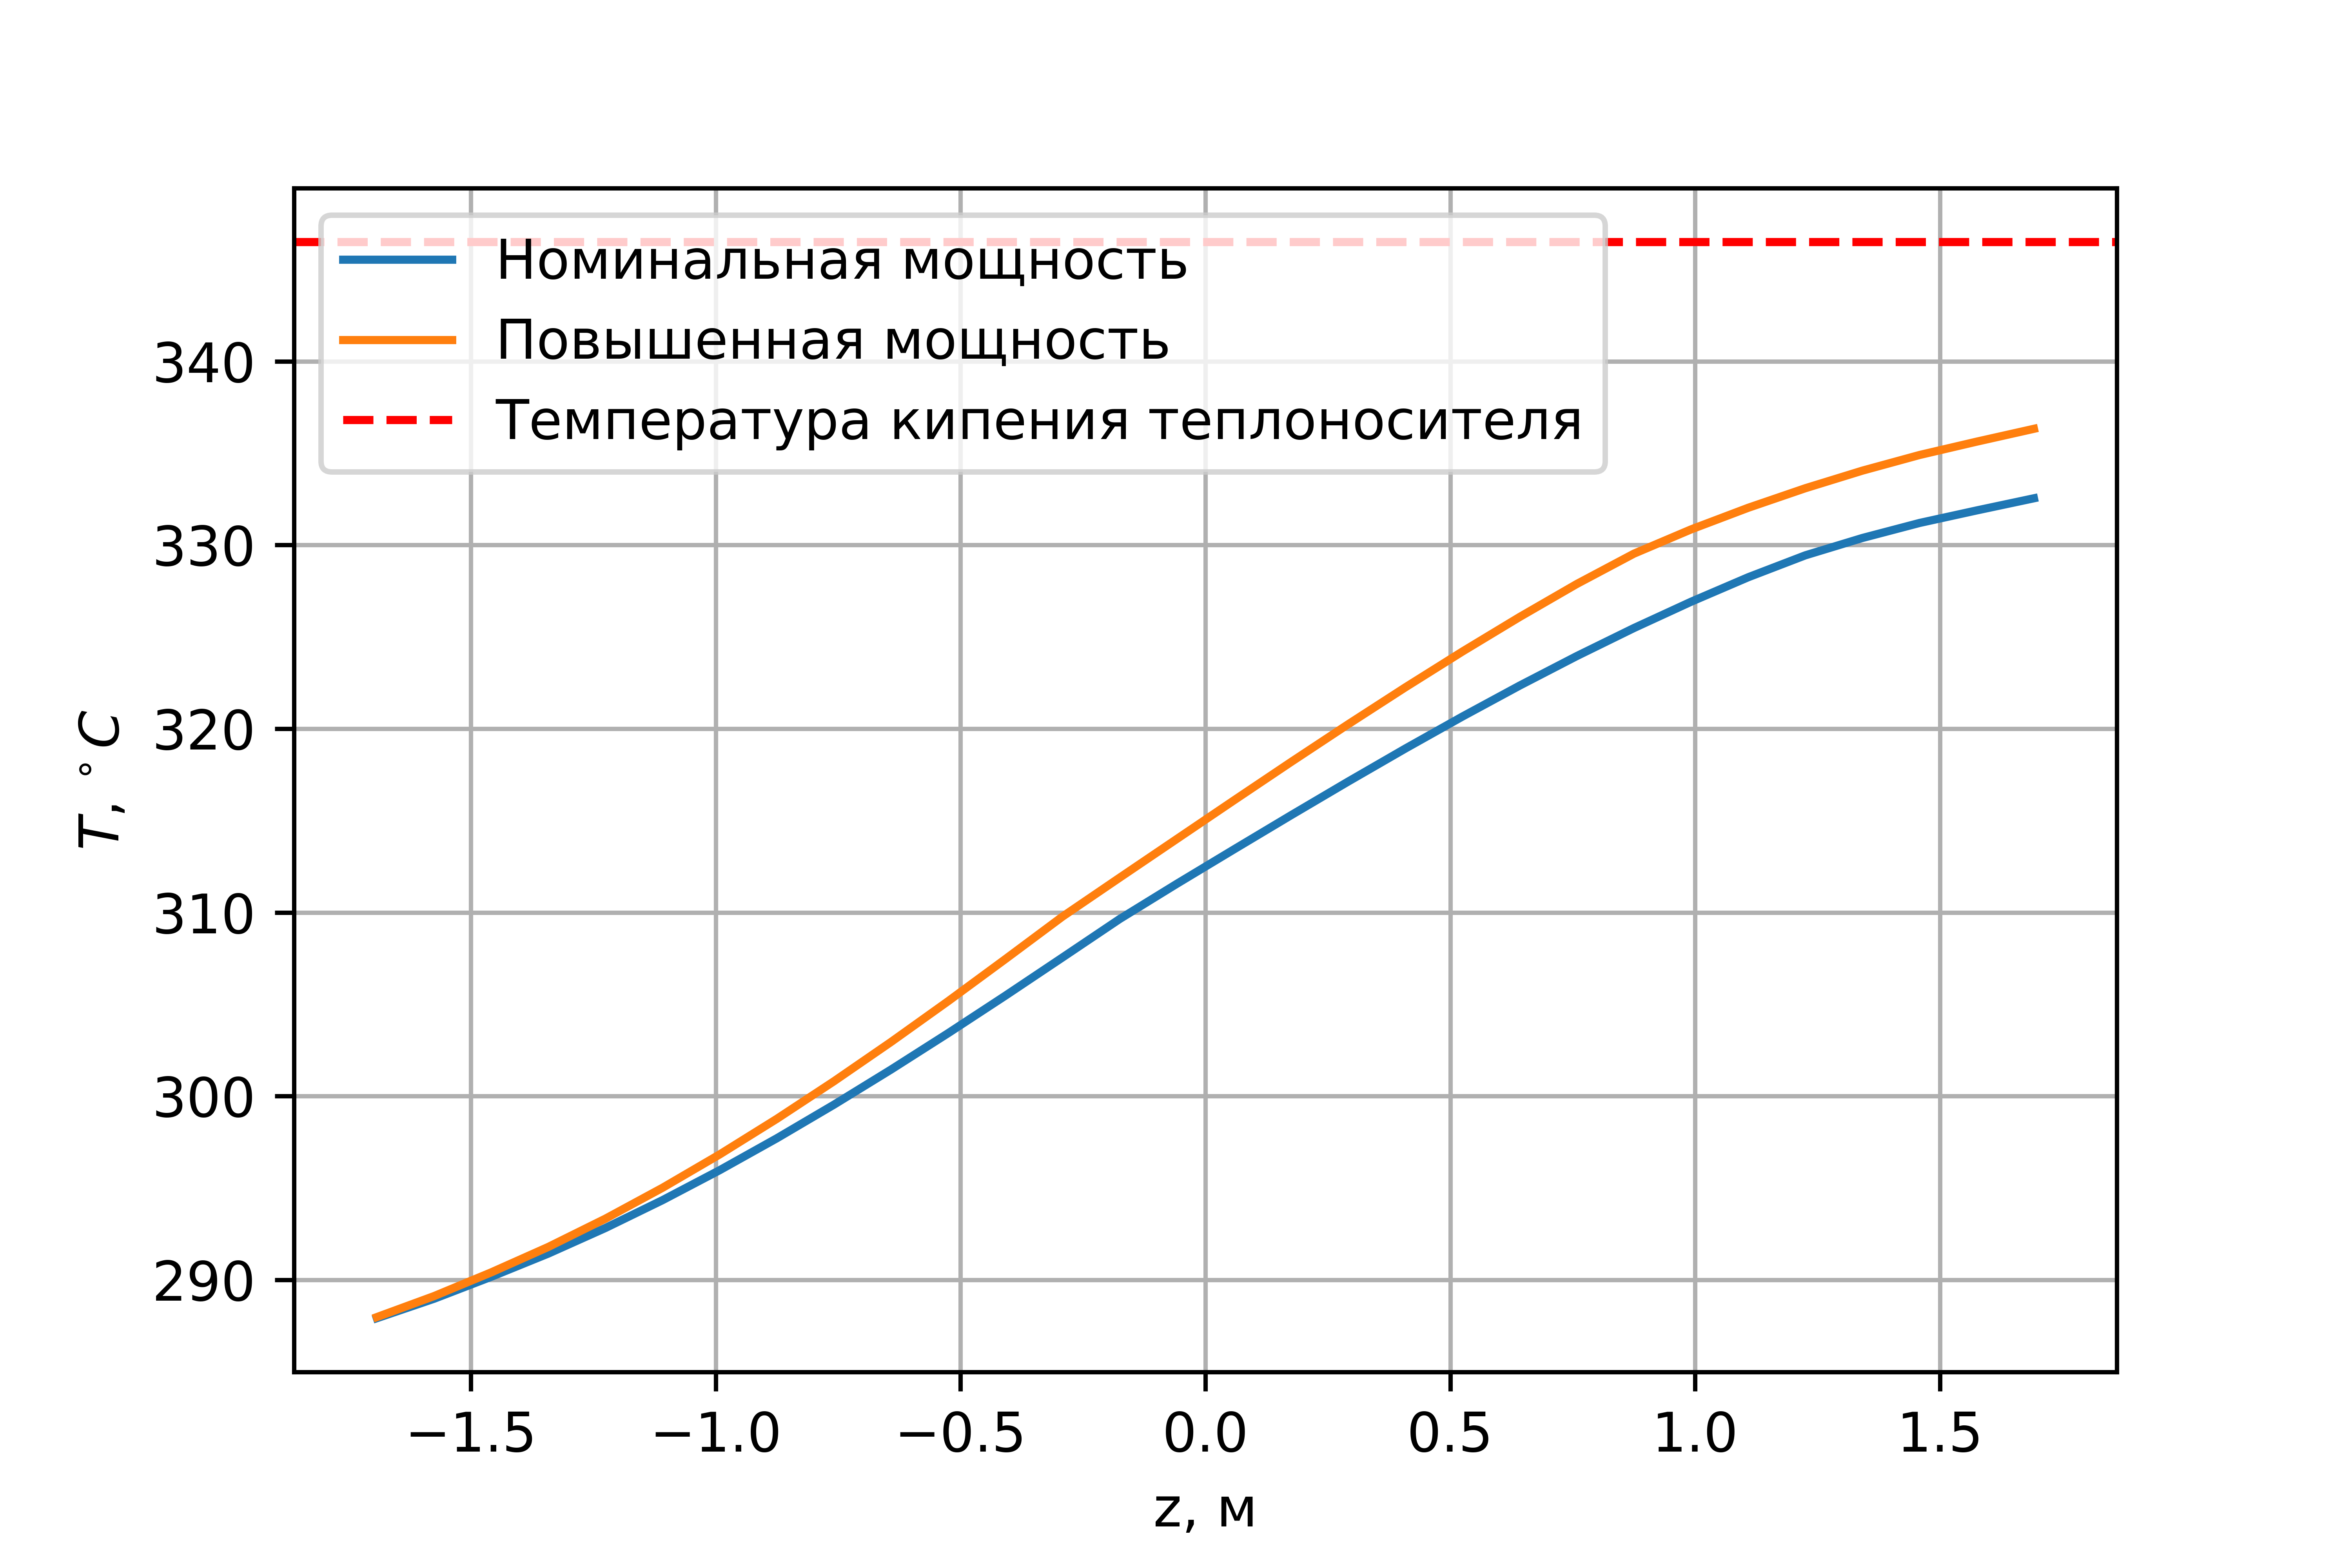
\includegraphics{treton_t_tepl_povish_compare.png}
		\caption{Распределение температуры теплоносителя по высоте АЗ}
		\label{pic:treton-t-tepl-povish-compare} % название для ссылок внутри кода
	\end{center}
\end{figure}

\begin{figure}[H]
	\begin{center}
		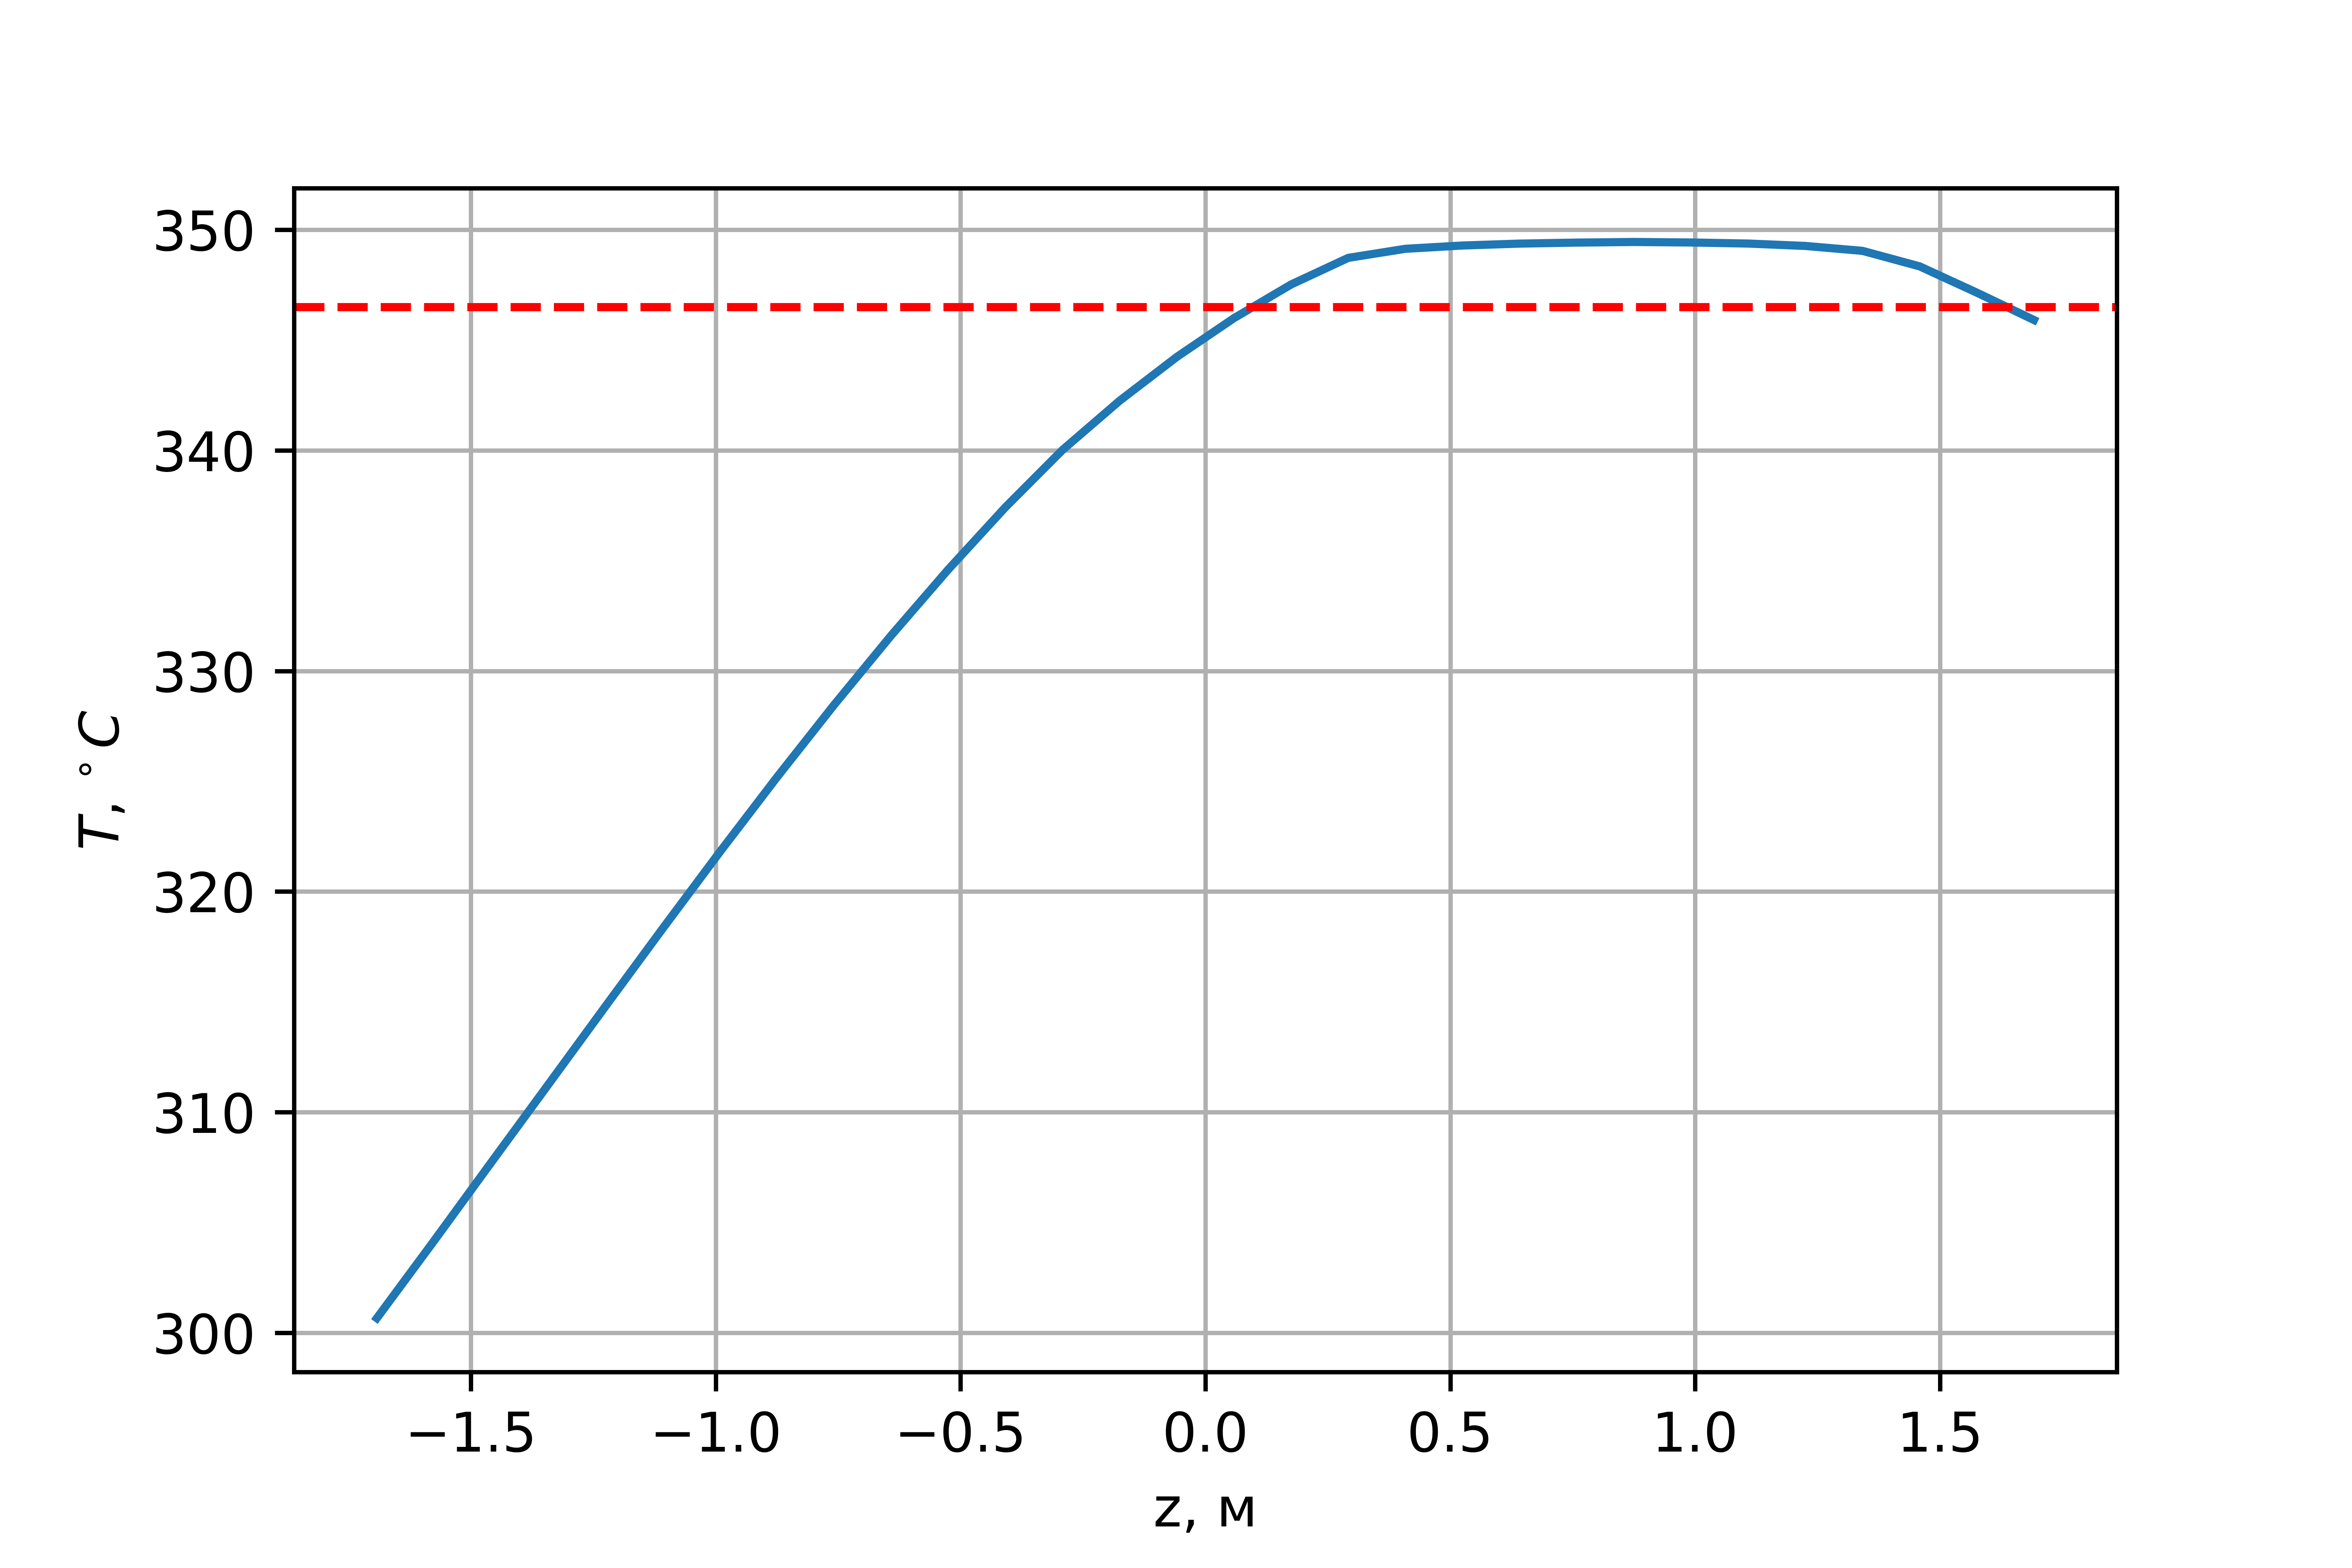
\includegraphics{treton_povish_obl_naruj_max.png}
		\caption{Распределение температуры наруженй оболочки твэлов по высоте для кассеты с максимальной температурой теплоносителя}
		\label{pic:treton-povish-obl-naruj-max} % название для ссылок внутри кода
	\end{center}
\end{figure}

из \ref{tabular:t_max_nominal_compare} видно, что при повышении мощности на 15\% наблюдается превышение запаса до кипения теплоносителя на 3.8 $^\circ C$, что не превышает температуры насыщения, однако для кассеты с максимальной температурой теплоносителя наблюдается пристеночное кипение вблизи оболочек твэлов. 
Для топлива превышение температуры составило 71.4 $^\circ C$, однако превышения критических для топлва температур не наблюдается. Общий график температур для работы реактора на повышенном уровне мощности представлен на рисунке \ref{pic:treton-povish-obl-tepl-obsh}

\begin{figure}[H]
	\begin{center}
		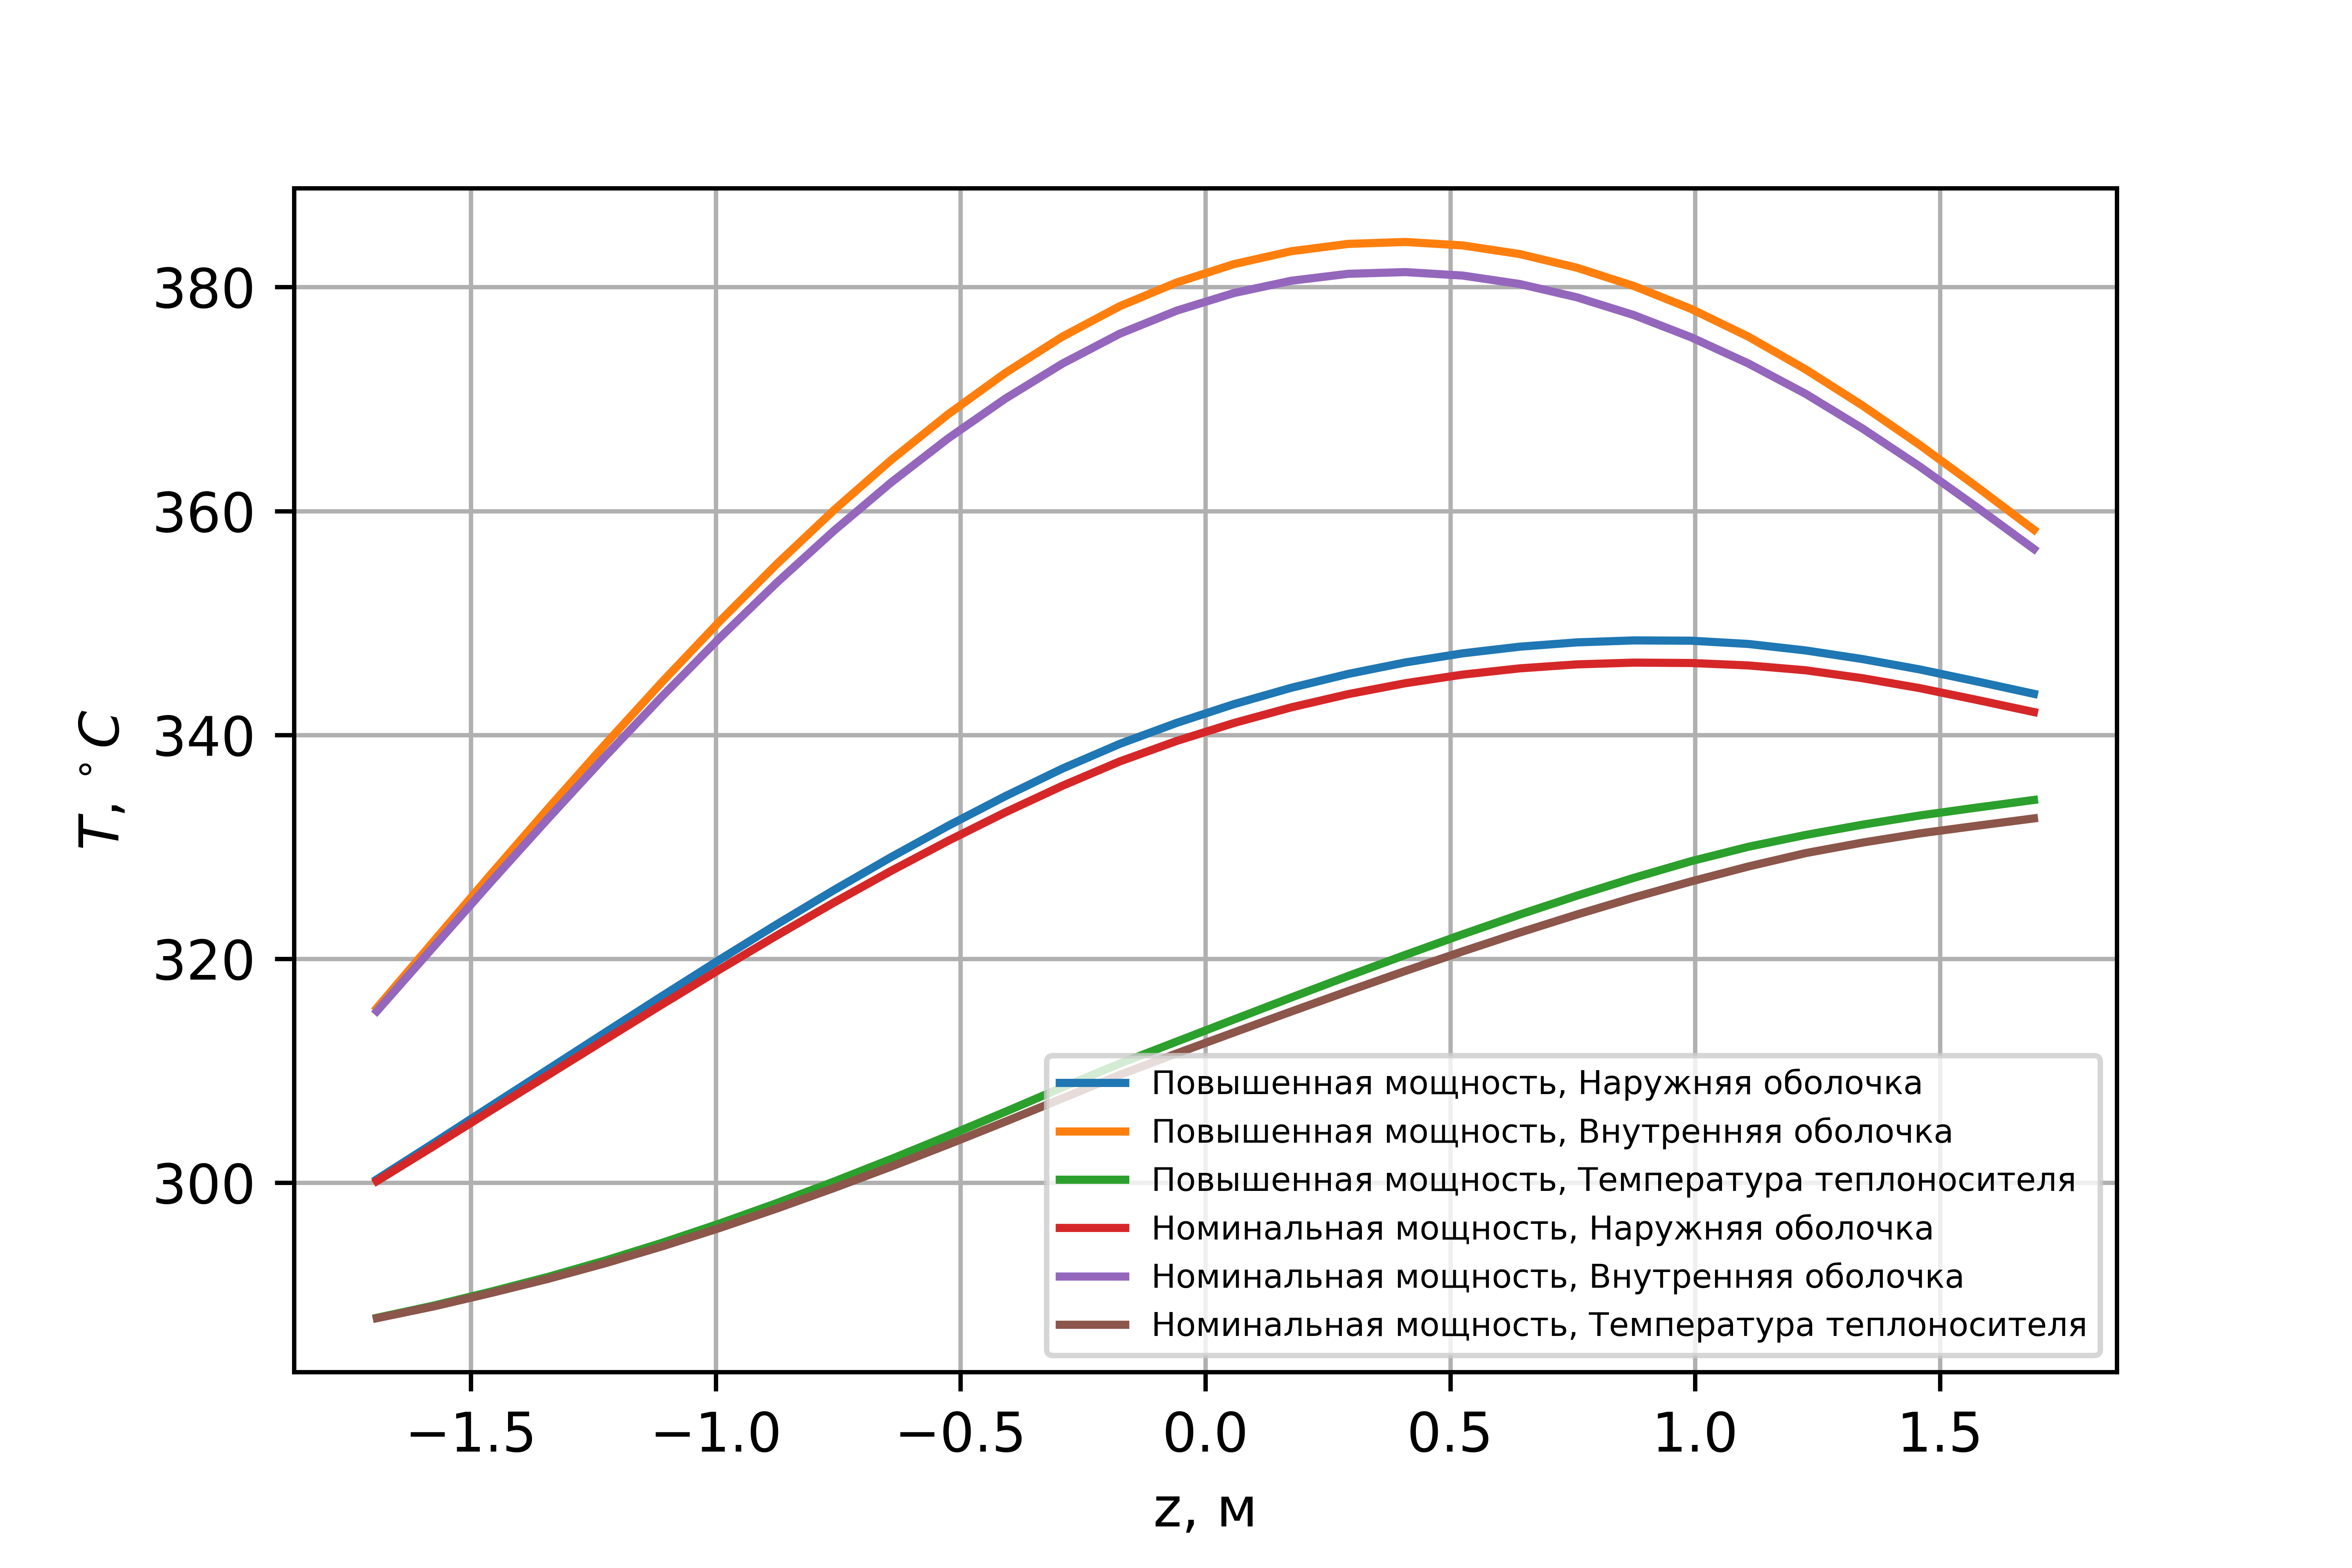
\includegraphics{treton_povish_obl_tepl_obsh.png}
		\caption{Распределение температур по высоте АЗ}
		\label{pic:treton-povish-obl-tepl-obsh} % название для ссылок внутри кода
	\end{center}
\end{figure}


На рисунке \ref{pic:p-povish-max} представлена зависимость давления в кассете с максимальной температурой от высоты. Для давления наблюдается превышение в центре ТВС на 4.3 КПа. 


\begin{figure}[H]
	\begin{center}
		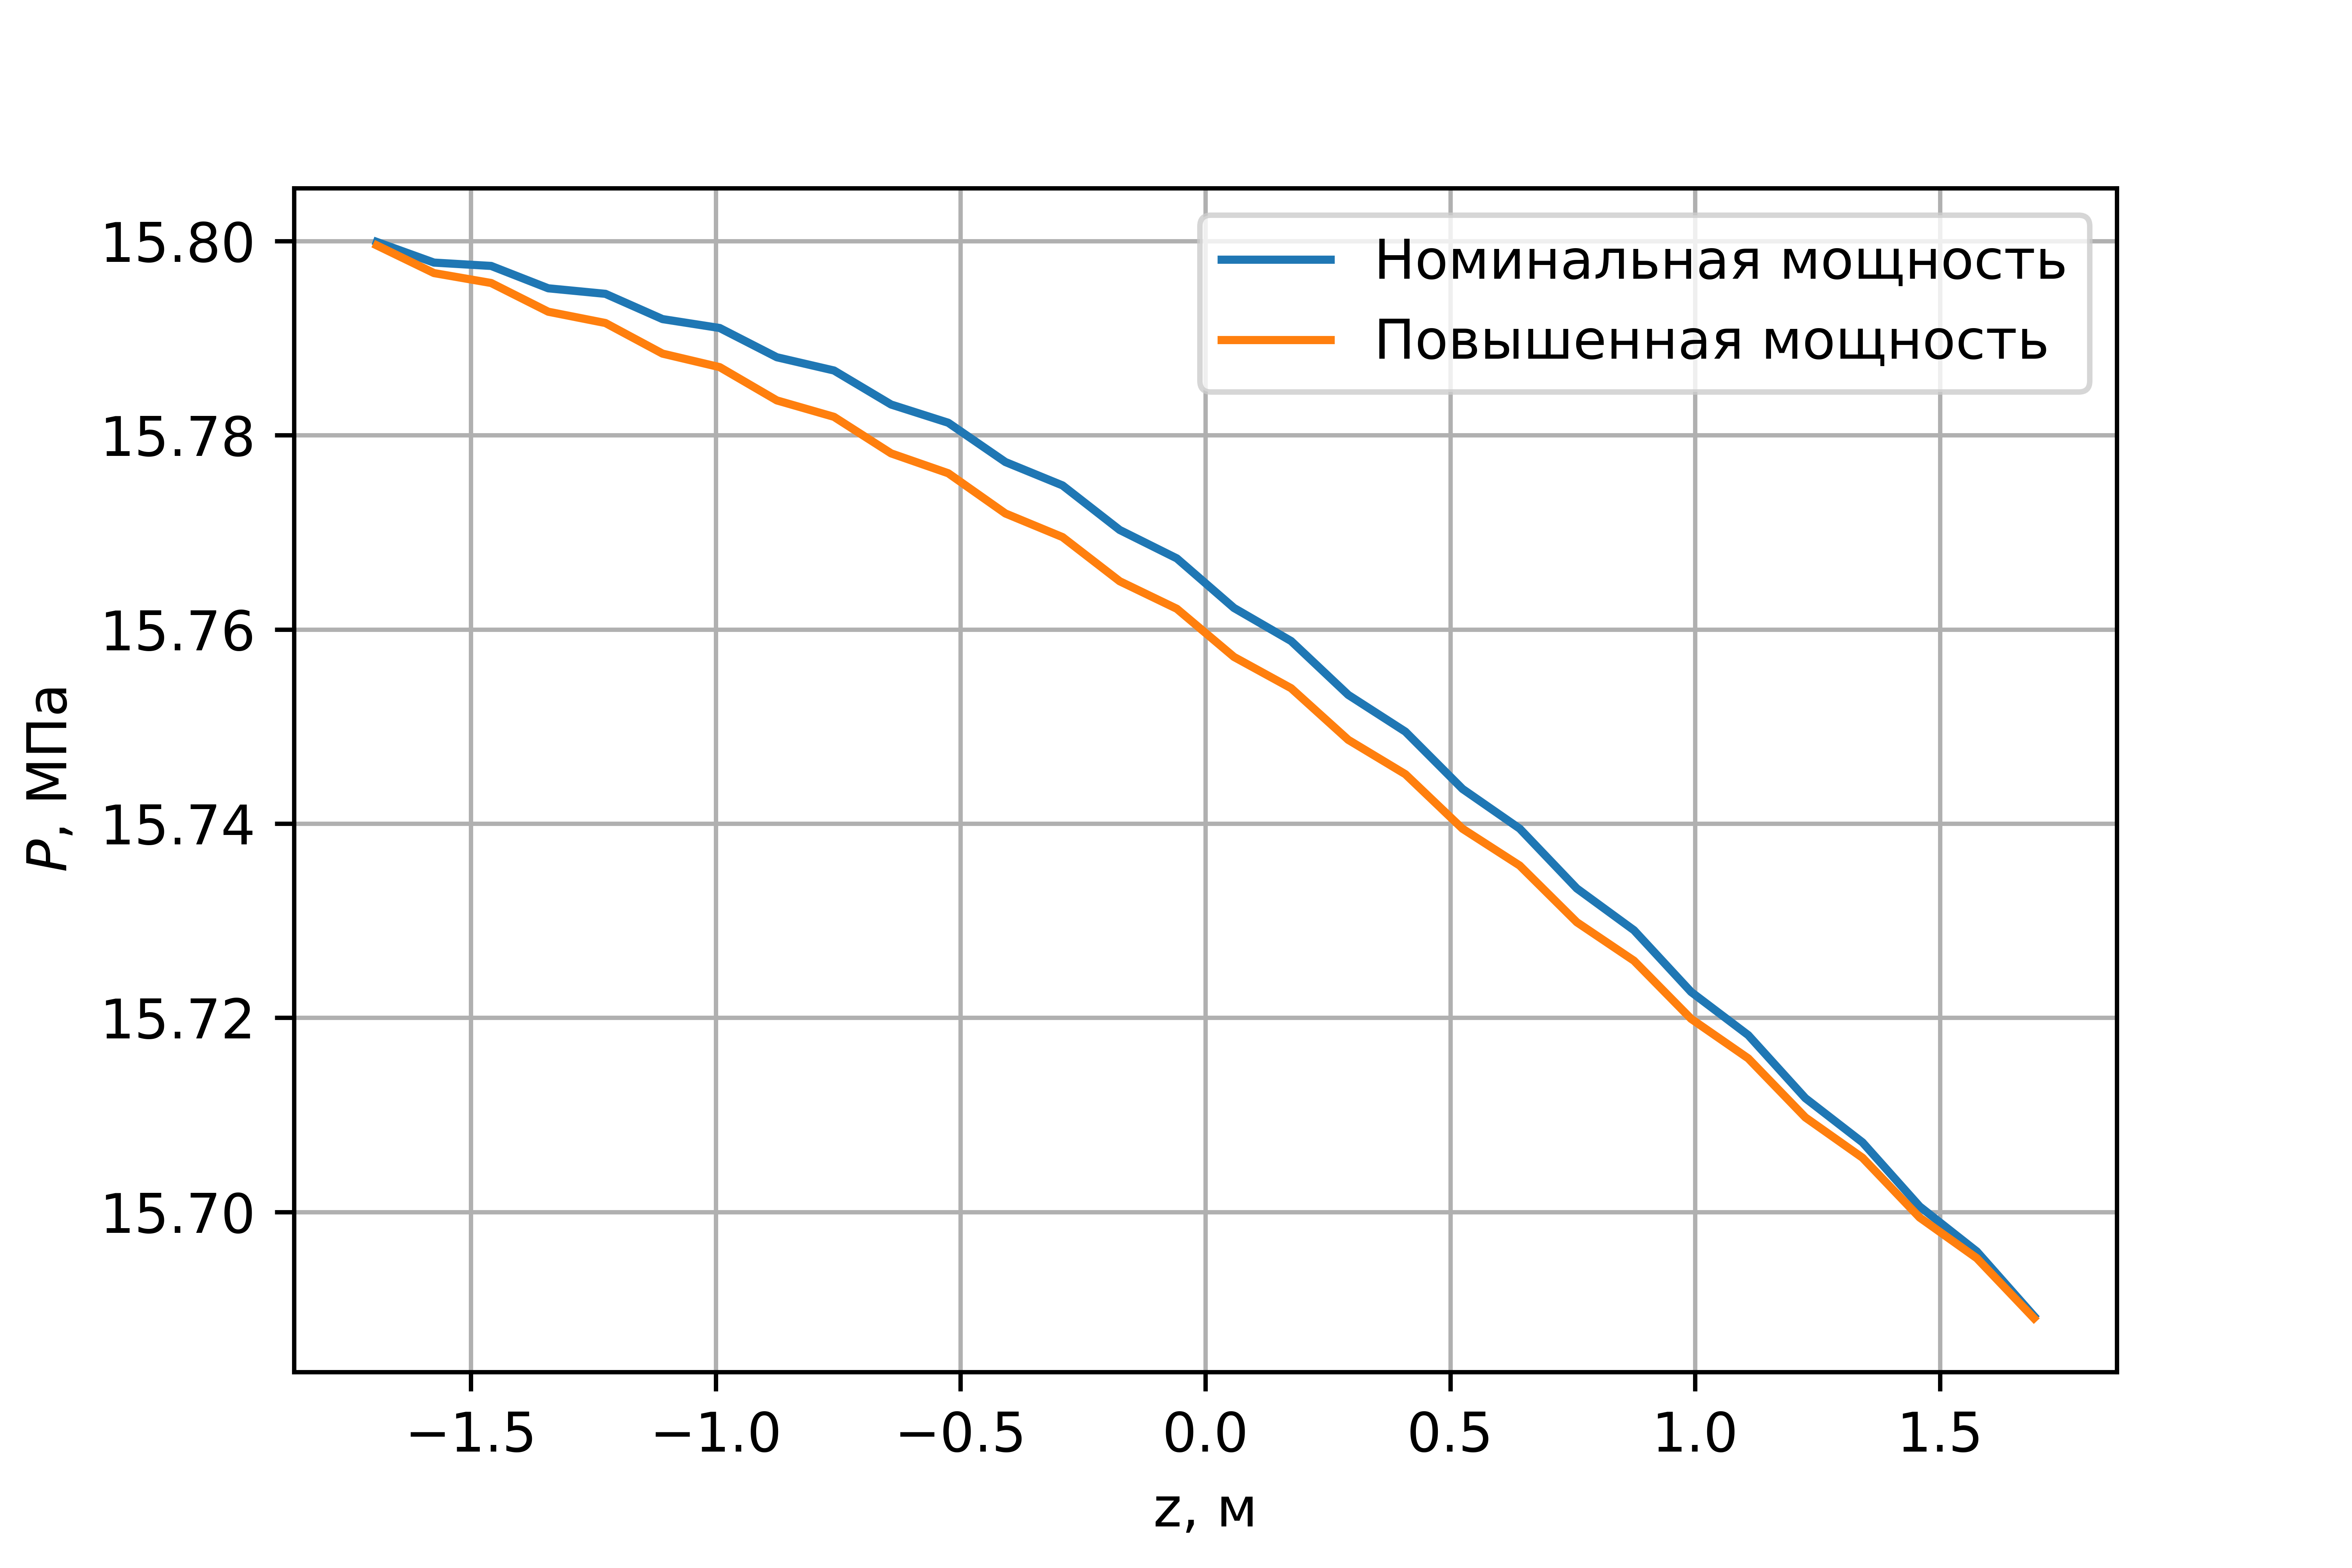
\includegraphics{p_povish_max.png}
		\caption{Распределение давления в кассете с максимальной температурой по высоте АЗ}
		\label{pic:p-povish-max} % название для ссылок внутри кода
	\end{center}
\end{figure}

Из рисунка \ref{pic:podogrev-povish} видно, что при повышении мощности на 15\% подогрев в центральной ТВС поднялся на 3.7 $^\circ C$, и на $3.4 ^\circ C$ в среднем по всем ТВС. На рисунке \ref{pic:podogrev-povish-by-r} представлено распределение подогревов, усредненных по радиальным группам ТВС


\begin{figure}[H]
	\begin{center}
		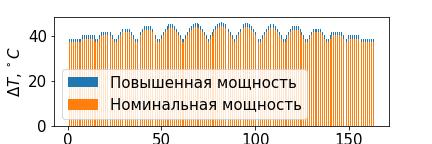
\includegraphics{podogrev_povish.jpg}
		\caption{Распределение подогревов по всем ТВС}
		\label{pic:podogrev-povish} % название для ссылок внутри кода
	\end{center}
\end{figure}

\begin{figure}[H]
	\begin{center}
		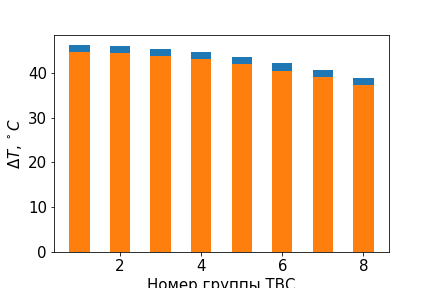
\includegraphics{podogrev_povish_by_r.png}
		\caption{Распределение подогревов по радиальным группам ТВС}
		\label{pic:podogrev-povish-by-r} % название для ссылок внутри кода
	\end{center}
\end{figure}


% TODO: сравнение расходов

\subsection{Расчет теплогидравлических характеристик при отключении одного ГЦН}
Для рассматриваемой установки были проведены расчеты основных теплогидравлических параметров в случае отключения одного из четырех ГЦН. Такой режим работы характерен сниженным уровнем мощности и расхода теплоносителя. При моделировании данного процесса был учтен возникающий при отключении петли возникающий обратный ток теплоносителя и его неполное перемешивание в напорной камере. В таком случае при отключении одного из ГЦН температура теплоносителя на входе снижается в петле где возникает обратный ток, а также в соседней с ней петле в следствие подмешивания холодного тока из нерабочей петли. 

С точки зрения расчетной модели для воспроизведения описанных условий была задана пониженная температура $T_{\text{in}}^{\text{low}}=284 \circ C$ на входе в захоложенные петли. Распределение номеров ячеек по четырем петлям ГЦН представлено на рисунке \ref{pic:treton-quarts}. Температура была снижена для ячеек, расположенных в левой верхней и левой нижней области по картограмме \ref{pic:treton-quarts} при задании во входном файле T\_IN.TXT расчетного модуля «ТРЕТОН». В файл Q6.TXT входное тепловыделение для всех ячеек было снижено на 25\% ввиду снижения мощности. 

По результатам расчета получены максимальные занчения температур топлива, оболочек и теплоносителя, которые представлены в таблице \ref{tabular:t_one_gcn_nominal_compare}